\section{Results}
\label{sec:results}

\subsection{Four families of evidence}
\label{subsec:families}

The empirical evidence in this paper comes from four \emph{families} of
study, each with a distinct methodological job
(\Cref{tab:dataset-families}). The families are not redundant
replications of the same experiment on different systems; they
\emph{stress different parts of the same thesis}, and we report them
\emph{separately} because their sampling protocols and cost dimensions
are not directly comparable. Aggregating across families would mix
incompatible sampling mechanisms; each per-RQ subsection below instead
walks through the evidence one family at a time.

\begin{itemize}
    \item \StudyReplication -- \emph{same published sampling studies,
    different cost model.} Replays the published \dsXmat corpus
    (with a $2\!\times\!2$ cost--target matrix over $17$ inputs) and
    seven Kaltenecker \etal{} systems under their original
    synthesis-based sampling traces, but with empirical cost in place
    of sample count. This family carries the historical continuity
    with the sampling literature; it is the spine of the
    contribution.
    \item \StudyEnergy -- \emph{same sampling question, different
    notion of cost.} Adds the performance--energy corpus / Green Configuration
    corpus, where two cost properties (\emph{performance} and
    \emph{energy}) are measured in parallel. This family tests whether
    the conclusions survive when ``cost'' means something other than
    runtime.
    \item \StudyWorkload -- \emph{same system, changing
    workload/input context.} Uses the \dsWLI corpus, $9$ systems
    each measured under multiple workloads (here
    $93$ system--workload contexts in total). This family stresses
    context sensitivity (RQ5) inside a single sampling protocol.
    \item \StudyLinux -- \emph{same thesis, extreme
    configuration-space scale.} Runs seven \dsTux releases (v4.13,
    v4.15, v4.20, v5.0, v5.04, v5.07, v5.08), under a custom pool-based
    subsampling
    protocol with storage-bound cost ($\mathit{cost}(c)$ $=$
    uncompressed binary size). The configuration space is one to two
    orders of magnitude larger than anywhere else in the paper, with
    a strategy panel (active learning, farthest-first diversity) that
    has no analogue in the other families.
\end{itemize}

\begin{table*}[t]
\centering
\caption{The four families of evidence. Each family has a distinct
methodological job; we report results separately and never aggregate
across families because the sampling protocols and cost dimensions are
not directly comparable.}
\label{tab:dataset-families}
\footnotesize
\setlength{\tabcolsep}{4pt}
\begin{tabular}{l p{0.18\linewidth} p{0.18\linewidth} p{0.20\linewidth} p{0.22\linewidth}}
\toprule
Family & What it tests & Datasets & Sampling protocol \& cost & Distinctive contribution / main caveat \\
\midrule
\StudyReplication
& Does empirical cost change conclusions of the published sampling literature?
& \dsXmat ($1{,}152$ configs, $17$ inputs); the Kaltenecker \etal{} corpus ($7$ systems, $|C|\!\in\![432,68k]$)
& Published sample traces (synthesis-based: random, t-wise, solver-based, Henard, distance-based, divDistBased); cost is the published time-like property
& Closest link to prior work; minimal protocol invention. Caveat: limited to published cost--target combinations; x264 matrix is one-system. \\
\midrule
\StudyEnergy
& Does the conclusion survive when cost is energy instead of runtime?
& the performance--energy corpus ($7$ systems, performance + energy)
& Generated sampling (random, balanced, diversity, pairwise, pilotCost + oracles); cost is performance \emph{or} energy ($2\!\times\!2$ scenarios per system)
& Cost is no longer synonymous with runtime. Caveat: sampling traces had to be regenerated; energy is one specific cost property and should not be over-generalized. \\
\midrule
\StudyWorkload
& Does the answer change when the same system runs under another workload/input?
& Workload-impact ICSE 2023 ($9$ systems $\times$ $93$ workload contexts; later: input-aware, YouTube UGC)
& Generated sampling over the measured universe; cost is wall-clock time (or oriented throughput); same system across many workloads
& Strongest direct support for context sensitivity (RQ5). Caveat: additional workload datasets are mostly diversification rather than a new claim. \\
\midrule
\StudyLinux
& Does the thesis hold at very large configuration-space scale?
& \dsTux v4.13 ($92{,}562$) -- v5.08 ($21{,}923$); seven releases under \texttt{randconfig}
& Custom pool-based subsampling (random, balanced, coverage, uncertainty, diversity + oracles); storage-bound cost ($\mathit{cost}(c) = $ \texttt{vmlinux} size)
& Unique large-space, high-feature, storage-cost stress test. Caveat: cost is size/storage, not runtime; protocol differs more from the trace-based families. \\
\bottomrule
\end{tabular}
\end{table*}

The four families share the same RQ structure and the same cost-model
formulation (\Cref{sec:cost_model}). What changes across families is
\emph{which assumption is being stressed}: \StudyReplication stresses the cost
abstraction itself, \StudyEnergy stresses the cost dimension, \StudyWorkload
stresses the input/workload context, and \StudyLinux stresses both scale and
the strategy panel. A finding that survives all four families is robust to the
abstraction, the dimension, the context, and the scale; a finding that
appears in only one family identifies a specific failure mode of the
size-as-cost abstraction.

\subsection{Reading guide}
\label{subsec:reading-guide}

Each per-RQ subsection below walks through the evidence one family at
a time, in fixed order: \StudyReplication, \StudyEnergy, \StudyWorkload, \StudyLinux, and
closes with a cross-family take-away box and a hypothesis-verdict
paragraph. \red{Numbers reported here come from a lightweight
ridge/log-linear learner; replication with stepwise linear regression
and CART is in progress and will be added before camera-ready.}

\Cref{tab:hypothesis-verdicts} reports the headline verdict on each of
the twelve hypotheses H1a--H5c stated in \Cref{sec:study_design}. Each
RQ subsection below pairs the descriptive numbers with the corresponding
hypothesis verdicts.

% Auto-generated by scripts/generate_hypotheses_table.py.
% Do not edit by hand; rerun the generator after updating the artifacts.
\begin{table*}[t]
\centering
\caption{Hypothesis verdicts. Each verdict is `$\checkmark$ supported',
`$\times$ refuted', or `$\circ$ inconclusive', followed by the count of
scopes (NewRuns systems for H1--H4, x264 inputs $\times$ scenarios for the matrix
column, workload-impact systems for the workload column, LCBench datasets
for the LCBench column, and seven Linux releases for the Linux column)
where the per-scope test agreed with the global label.
Statistical tests and thresholds are in the third column. H3b and H5b are
global tests (one scope each). The workload-impact column only contributes
RQ5 evidence, since it was added specifically to test workload sensitivity
across nine systems and $93$ workloads. The LCBench column contributes
H1--H4 workload-level verdicts on $35$ dataset contexts and study-level
RQ5 verdicts for the non-pure-software external-validation family. For the RQ5 rows specifically,
the x264 column reports \emph{scenario-level} verdicts on one system
(four cost$\times$target scenarios, each aggregating over $17$ input videos),
whereas the workload-impact column reports \emph{system-level} verdicts
(nine systems, each aggregating over $6$--$13$ workloads), and the
LCBench column reports a \emph{study-level} verdict aggregating over
$35$ dataset contexts.
Linux is reported separately rather than aggregated because of its different
protocol and strategy panel (\Cref{sec:results}); H2b refutes on
Linux at the aggregate median because the per-strategy ratios average to
$\sim\!\!1.00$, but the per-strategy decomposition shows two strategies
(\texttt{diversity}, \texttt{uncertainty}) clearly miscalibrated. The
size-as-cost effect (H5b) is borderline at the by-target average
($\Delta$ flip-rate $= 0.042$) but the asymmetric scenario alone
(cost$=$time, target$=$size) shows a $13$-pp jump
(\Cref{tab:x264-matrix-summary}).}
\label{tab:hypothesis-verdicts}
\scriptsize
\setlength{\tabcolsep}{3pt}
\begin{tabular}{l l p{4.2cm} p{3.2cm} c c c c c}
\toprule
ID & RQ & Claim & Test / threshold & NewRuns & \shortstack{x264 matrix \\ inputs} & \shortstack{Workload-impact \\ workloads} & \shortstack{LCBench \\ datasets} & Linux \\
\midrule
\textbf{H1a} & RQ1 & Per-config.\ cost CV is non-negligible. & $\mathrm{CV}\geq 0.20$ or $p_{90}/p_{10}\geq 1.5$ & $\checkmark$\,6/7 & $\checkmark$\,22/34 & -- & $\checkmark$\,35/35 & $\checkmark$\,7/7 \\
\textbf{H1b} & RQ1 & Strategies differ in $\TrainCost$ at fixed $n$. & Kruskal--Wallis $p<0.05$ and $\eta^2\geq 0.01$ & $\checkmark$\,7/7 & $\checkmark$\,34/34 & -- & $\checkmark$\,35/35 & $\checkmark$\,7/7 \\
\textbf{H2a} & RQ2 & $n$ is positively rank-correlated with $\TrainCost$. & Spearman $\rho>0$, $p<0.05$ & $\checkmark$\,7/7 & $\checkmark$\,34/34 & -- & $\checkmark$\,35/35 & $\checkmark$\,7/7 \\
\textbf{H2b} & RQ2 & Calibration ratio $\Ratio$ is not centered at $1$. & $95\%$ bootstrap CI of median excludes $1$, $|\widetilde{\Ratio}-1|\geq 0.05$ & $\circ$\,3/7 & $\circ$\,0/34 & -- & $\checkmark$\,31/35 & $\times$\,0/7 \\
\textbf{H2c} & RQ2 & Calibration depends on sampling strategy. & Kruskal--Wallis of $\Ratio$ across strategies, $p<0.05$ & $\checkmark$\,7/7 & $\checkmark$\,34/34 & -- & $\checkmark$\,35/35 & $\checkmark$\,7/7 \\
\textbf{H3a} & RQ3 & Rankings under count vs.\ measured cost diverge. & $\geq 1$ top-$1$ flip across cost weights & $\checkmark$\,3/7 & $\checkmark$\,25/68 & -- & $\checkmark$\,33/35 & $\checkmark$\,7/7 \\
\textbf{H3b} & RQ3 & Divergence is stronger when cost CV is high. & Spearman(CV, flips/$7$) across systems & $\checkmark$\,1/1 & -- & -- & -- & -- \\
\textbf{H4a} & RQ4 & Some $(s,n)$ combinations are Pareto-efficient under one cost only. & $\geq 1$ combination only on count or only on measured-cost front & $\checkmark$\,5/7 & $\checkmark$\,65/68 & -- & $\checkmark$\,32/35 & $\checkmark$\,7/7 \\
\textbf{H4b} & RQ4 & Measured-cost frontier differs from count frontier. & Jaccard$<1$ & $\checkmark$\,5/7 & $\checkmark$\,65/68 & -- & $\checkmark$\,32/35 & $\checkmark$\,7/7 \\
\textbf{H5a} & RQ5 & Validity depends on input/workload within a fixed system. & Kruskal--Wallis of $\Ratio$ across inputs/workloads within a system & -- & $\checkmark$\,2/4 & $\checkmark$\,5/9 & $\checkmark$\,1/1 & -- \\
\textbf{H5b} & RQ5 & Size-as-cost gap differs by predicted property on x264. & $|\Delta\text{flip-rate}|\geq 0.05$ & -- & $\circ$\,0/1 & -- & -- & -- \\
\textbf{H5c} & RQ5 & Measured-cost rankings less stable than count under context changes. & mean Kendall $\tau<0.95$ or median Jaccard$<0.9$ & -- & $\checkmark$\,1/1 & $\checkmark$\,9/9 & $\checkmark$\,1/1 & -- \\
\bottomrule
\end{tabular}
\end{table*}


The reference tables for the four families are
\Cref{tab:systems-and-cost} (\StudyReplication),
\Cref{tab:x264-matrix-summary} (\StudyReplication/x264 $2\!\times\!2$),
\Cref{tab:twins-summary} (\StudyEnergy),
\Cref{tab:workload-impact-meta} (\dsWLI), and
\Cref{tab:linux-summary} (\StudyLinux). Aggregate numbers can be misleading
on their own, so each RQ subsection pairs the family-level aggregate
with two \emph{contrasting extremes} picked from the same data: the
case where the size-as-cost abstraction breaks the most for that RQ,
and the case where it essentially holds. These vignettes are bookends,
not the statistical median.

\begin{table*}[t]
\centering
\caption{\StudyReplication -- configurable systems used in the
cross-system results, with metadata and key empirical signals at a
glance. JavaGC and VP9 are part of the Tier-2A corpus but not yet
included in this batch; x264 is reported separately
(\Cref{tab:x264-matrix-summary}).}
\label{tab:systems-and-cost}
\footnotesize
\setlength{\tabcolsep}{4.5pt}
\begin{tabular}{l l r r l r r r r r r}
\toprule
System  & Domain & $|C|$ & $|O|$ & Target perf. & Cost CV & $p_{90}/p_{10}$ & Spearman & med.\ \%cost/\%n & flips/$7$ & Jaccard \\
\midrule
LLVM        & Compiler            & $1{,}024$    & $11$ & Compilation time & $0.072$ & $1.21$  & $0.943$ & $0.996$ & $0$ & $0.333$ \\
Polly       & Code optimizer      & $59{,}897$\rlap{$^{*}$} & $40$ & Runtime          & $0.239$ & $2.08$  & $0.943$ & $0.997$ & $0$ & $0.500$ \\
Dune        & Multigrid solver    & $2{,}304$    & $32$ & Solving time     & $0.344$ & $1.83$  & $0.943$ & $1.011$ & $0$ & $1.000$ \\
HIPAcc      & Image processing    & $13{,}485$   & $54$ & Solving time     & $0.435$ & $2.59$  & $0.943$ & $1.056$ & $0$ & $1.000$ \\
7Z          & File archive        & $68{,}640$   & $44$ & Compression time & $1.188$ & $10.13$ & $0.943$ & $0.955$ & $1$ & $0.429$ \\
BerkeleyDBC & Embedded DB         & $2{,}560$    & $18$ & Response time    & $1.420$ & $47.90$ & $0.879$ & $0.797$ & $1$ & $0.600$ \\
lrzip       & File archive        & $432$        & $19$ & Compression time & $1.981$ & $47.04$ & $0.937$ & $0.856$ & $5$ & $0.600$ \\
\bottomrule
\multicolumn{11}{l}{\footnotesize $^{*}$ Polly: $59{,}897/60{,}000$ valid configurations reconstructed from the sampled CSVs.}
\end{tabular}
\end{table*}

\begin{table}[t]
\centering
\caption{\StudyReplication/x264 -- $2\times 2$ summary (cost property
$\times$ target property, aggregated across $17$ inputs).
Top-$1$ flips/$119$ counts the $(\text{input},\lambda)$ cases where
count-cost and empirical-cost rankings disagree at top-$1$;
Top-$1$ agree is the corresponding agreement fraction;
Kendall $\tau$ is the mean rank correlation;
Pareto Jaccard is the median frontier overlap. The
$(\text{cost}=\text{time}, \text{target}=\text{size})$ row is expanded
per-input in \Cref{tab:x264-per-input}.}
\label{tab:x264-matrix-summary}
\footnotesize
\setlength{\tabcolsep}{4.5pt}
\begin{tabular}{l l r r r r}
\toprule
Cost & Target & Top-$1$ flips/$119$ & Top-$1$ agree & Kendall $\tau$ & Pareto Jaccard \\
\midrule
time & time   & $6$  & $0.950$ & $0.916$ & $0.429$ \\
time & size   & $21$ & $0.824$ & $0.863$ & $0.375$ \\
size & time   & $13$ & $0.891$ & $0.951$ & $0.429$ \\
size & size   & $8$  & $0.933$ & $0.924$ & $0.500$ \\
\bottomrule
\end{tabular}
\end{table}

\begin{table*}[t]
\centering
\caption{\StudyEnergy -- representative pass over seven systems
($100$ seeds each, four cost-target scenarios per system).
\emph{Cost CV} and \emph{Spearman} ranges span the two cost
properties; \emph{med.\ \%cost/\%n} is the per-(system, cost)
calibration ratio range; \emph{Top-$1$ agree} ranges are over the
four cost-target scenarios per system. A top-$1$ agreement of $0$
means count-cost and empirical-cost rankings disagree at every
$\lambda$ for that scenario.}
\label{tab:twins-summary}
\footnotesize
\setlength{\tabcolsep}{4.5pt}
\begin{tabular}{l r r r r r}
\toprule
System & $|C|$ & Cost CV (range) & Spearman (range) & med.\ \%cost/\%n (range) & Top-$1$ agree (range) \\
\midrule
PostgreSQL ($11.2$) & $864$    & $0.058$--$0.068$ & $0.996$         & $0.999$         & $0.857$--$1.000$ \\
MongoDB             & $6{,}840$ & $0.142$--$0.167$ & $0.981$         & $0.996$--$0.997$ & $0.714$         \\
HSQLDB              & $864$    & $0.319$--$0.358$ & $0.991$         & $0.993$--$0.995$ & $0.429$--$0.857$ \\
x264                & $4{,}608$ & $0.413$--$0.595$ & $0.952$--$0.974$ & $0.976$--$0.984$ & $0.286$--$0.429$ \\
brotli ($1.0.7$)    & $180$    & $1.974$--$2.092$ & $0.890$--$0.896$ & $1.034$--$1.035$ & $0.000$--$1.000$ \\
lrzip               & $5{,}184$ & $2.003$--$2.180$ & $0.710$--$0.725$ & $0.824$--$0.842$ & $0.429$--$0.714$ \\
jump3r              & $4{,}296$ & $5.538$--$7.104$ & $0.749$--$0.835$ & $0.168$--$0.358$ & $0.000$--$0.429$ \\
\bottomrule
\end{tabular}
\end{table*}

\begin{table}[t]
\centering
\caption{\dsWLI -- meta-analysis over the ICSE 2023
workload corpus ($9$ systems, $93$ workload contexts). Pooled support
is a random-effects support rate over workload-level hypothesis
verdicts; $I^2$ quantifies how much the support rate varies across
systems. Within-system ranges in cost CV ($0.026$ to $2.367$) and
top-$1$ flips ($0$ to $7$ across $\lambda$ values) confirm that
workload changes both magnitude and decision verdict.}
\label{tab:workload-impact-meta}
\footnotesize
\setlength{\tabcolsep}{4.5pt}
\begin{tabular}{l r r l}
\toprule
Hypothesis & pooled support & $I^2$ & Reading \\
\midrule
\textbf{H1a} & $0.86$ & $0.59$ & mostly robust \\
\textbf{H1b} & $0.88$ & $0.41$ & mostly robust \\
\textbf{H2a} & $\mathbf{0.95}$ & $\mathbf{0.00}$ & robust across workloads \\
\textbf{H2b} & $0.33$ & $0.76$ & workload-sensitive \\
\textbf{H2c} & $0.90$ & $0.29$ & mostly robust \\
\textbf{H3a} & $0.80$ & $0.69$ & workload-sensitive \\
\textbf{H4b} & $0.81$ & $0.73$ & workload-sensitive \\
\bottomrule
\end{tabular}
\end{table}

\begin{table*}[t]
\centering
\caption{\StudyLinux -- cross-version summary across the seven
TuxKConfig releases. All seven share the storage-bound cost construct
and the same \texttt{randconfig}-induced sampling distribution; they
differ in pool size ($\sim\!\!5\!\times$ range) and in the heaviness
of the cost tail. The seven-release replication tightens three
findings: cost-blind samplers (\texttt{random}, \texttt{balanced},
\texttt{coverage}) are calibrated within $\pm\!0.7\%$ of $1$ on
\emph{every} pool; \texttt{diversity} drifts to a $[2.00, 2.28]$
window on every pool; \texttt{uncertainty}'s aggregate median is
direction-stable but pool-dependent (cheap at small $n$, expensive
at large $n$ on every release).}
\label{tab:linux-summary}
\footnotesize
\setlength{\tabcolsep}{4.5pt}
\begin{tabular}{l r r r r r r r}
\toprule
                              & v4.13       & v4.15       & v4.20       & v5.0        & v5.04       & v5.07       & v5.08       \\
\midrule
Pool size $|C|$               & $92{,}562$  & $39{,}391$  & $23{,}489$  & $\mathbf{19{,}952}$ & $25{,}847$  & $20{,}159$  & $21{,}923$  \\
Retained options              & $495$       & $497$       & $494$       & $494$       & $494$       & $494$       & $494$       \\
$\mathit{cost}(c)$ (median)   & $31$\,MB    & $64$\,MB    & $64$\,MB    & $68$\,MB    & $87$\,MB    & $88$\,MB    & $71$\,MB    \\
$\mathit{cost}(c)$ (max)      & $1.78$\,GB  & $1.87$\,GB  & $\mathbf{2.13}$\,GB & $1.96$\,GB & $2.05$\,GB & $2.00$\,GB  & $2.00$\,GB  \\
Cost CV                       & $\mathbf{1.43}$ & $1.16$  & $1.16$      & $1.12$      & $1.08$      & $\mathbf{0.99}$ & $1.01$  \\
$p_{90}/p_{10}$               & $4.61$      & $\mathbf{6.04}$ & $5.80$ & $5.70$      & $5.21$      & $4.76$      & $4.02$      \\
\midrule
\multicolumn{8}{l}{Per-strategy median calibration ratio} \\
\midrule
\texttt{random}               & $0.999$     & $1.003$     & $1.002$     & $1.002$     & $1.000$     & $0.999$     & $0.999$     \\
\texttt{balanced}             & $0.999$     & $1.000$     & $0.998$     & $0.998$     & $0.999$     & $0.997$     & $0.999$     \\
\texttt{coverage}             & $0.974$     & $1.007$     & $1.001$     & $0.997$     & $0.993$     & $0.993$     & $0.994$     \\
\texttt{uncertainty}          & $1.246$     & $0.996$     & $0.943$     & $0.979$     & $0.878$     & $0.839$     & $0.946$     \\
\texttt{diversity}            & $\mathbf{2.281}$ & $\mathbf{2.234}$ & $\mathbf{2.269}$ & $\mathbf{2.056}$ & $\mathbf{2.087}$ & $\mathbf{1.999}$ & $\mathbf{2.019}$ \\
\texttt{cheapOracle}          & $0.292$     & $0.248$     & $0.260$     & $0.261$     & $0.254$     & $0.270$     & $0.319$     \\
\texttt{expensiveOracle}      & $5.640$     & $4.955$     & $4.877$     & $4.765$     & $4.579$     & $4.193$     & $4.199$     \\
\midrule
Top-$1$ rank flips / $7$      & $2/7$       & $2/7$       & $2/7$       & $2/7$       & $\mathbf{7/7}$ & $\mathbf{4/7}$ & $\mathbf{6/7}$ \\
Count Pareto $|F|$            & $5$         & $6$         & $5$         & $5$         & $5$         & $5$         & $4$         \\
Empirical Pareto $|F|$        & $\mathbf{11}$ & $8$       & $7$         & $7$         & $8$         & $7$         & $8$         \\
Pareto Jaccard                & $0.45$      & $0.625$    & $\mathbf{0.71}$ & $\mathbf{0.71}$ & $0.50$  & $\mathbf{0.71}$ & $0.50$      \\
\bottomrule
\end{tabular}
\end{table*}

\subsection{RQ1 -- Empirical Cost Heterogeneity}
\label{subsec:results-rq1}

\paragraph*{\StudyReplication.}
\Cref{fig:rq1-heterogeneity} reports per-configuration cost spread for
the seven \StudyReplication systems, and \Cref{tab:systems-and-cost} gives the
underlying numbers. Cost CV ranges from $0.072$ (LLVM) to $1.981$
(lrzip), and $p_{90}/p_{10}$ reaches $47.9$ on BerkeleyDBC and $47.0$
on lrzip --- a single system can have its $90$th-percentile
configuration cost almost two orders of magnitude more than its
$10$th-percentile configuration. At the other end, LLVM is nearly
homogeneous ($p_{90}/p_{10}\!=\!1.21$). On x264, per-configuration cost
CV ranges $0.21$--$0.39$ across the $17$ inputs depending on
cost-target scenario.

\begin{figure}[t]
\centering
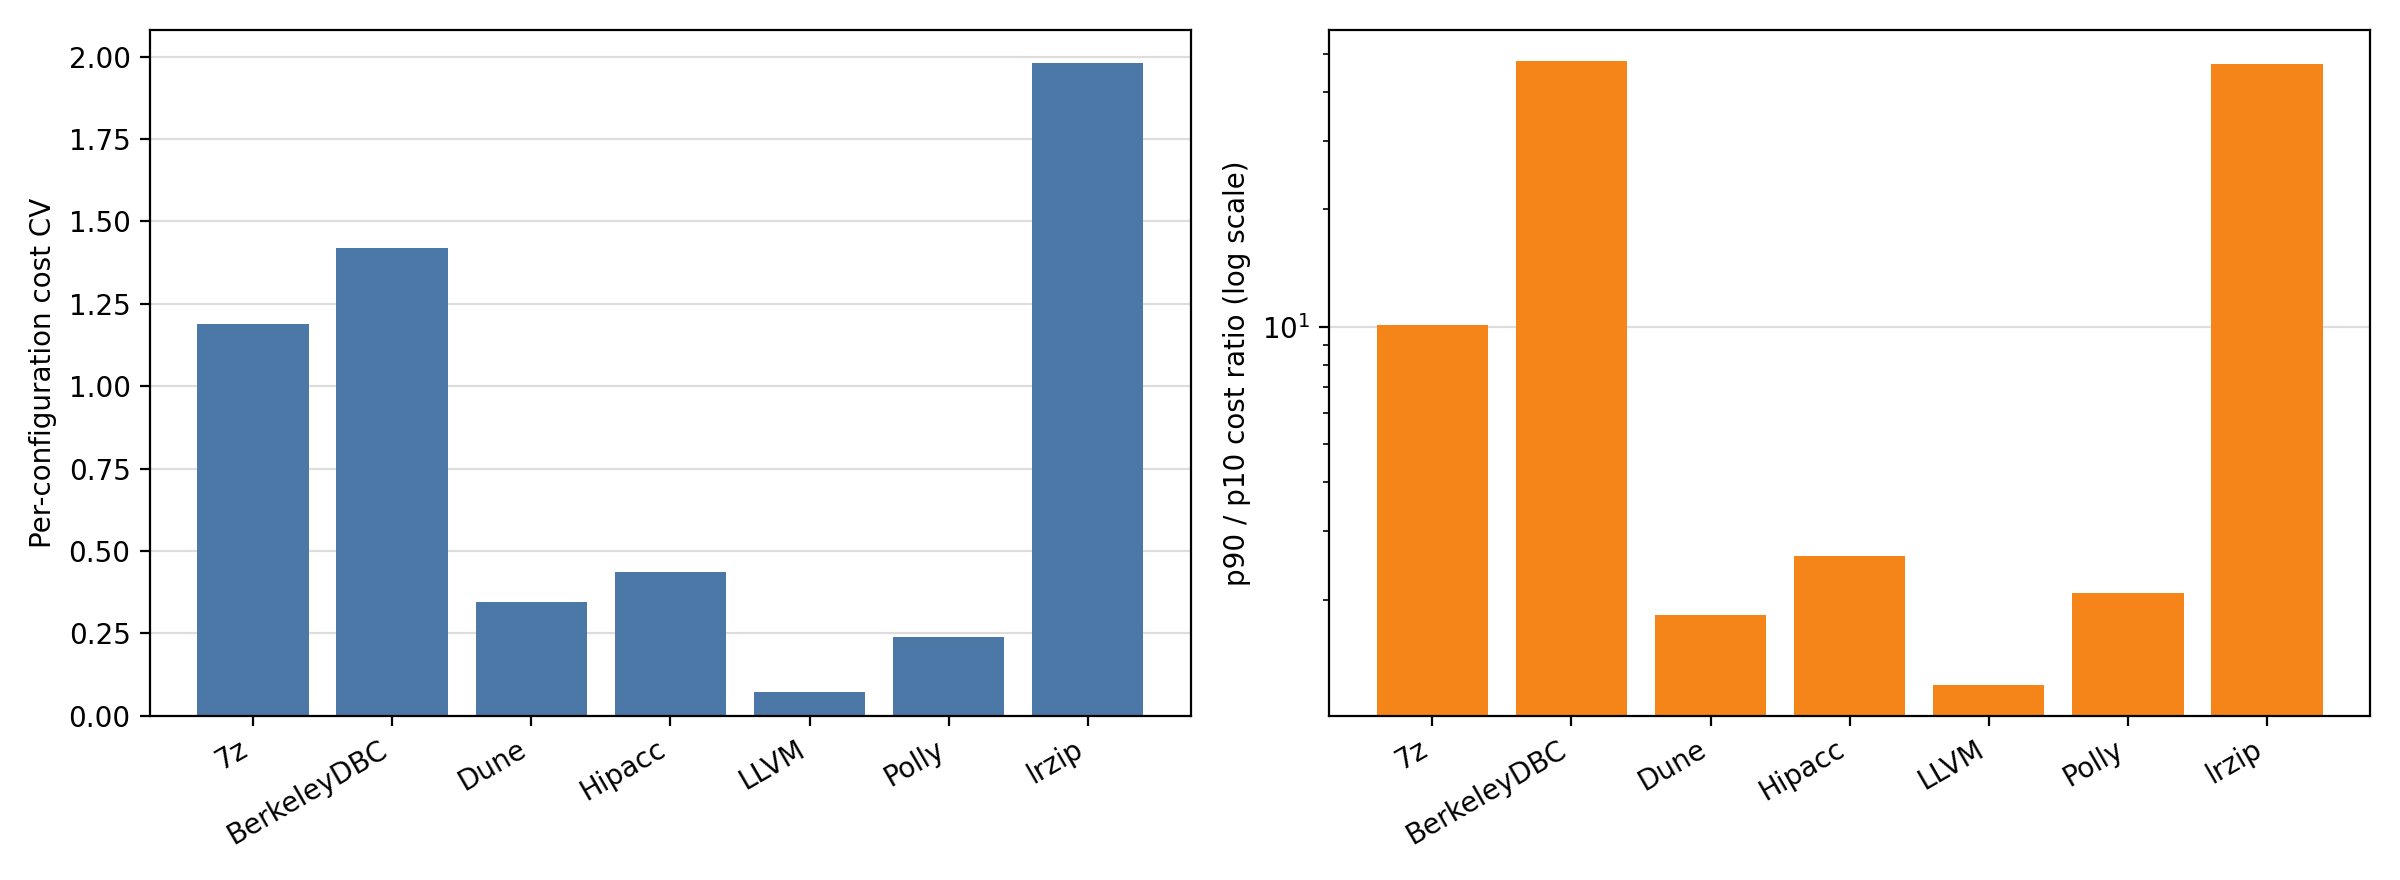
\includegraphics[width=\linewidth]{pic/results/fig_rq1_cost_heterogeneity_by_system.png}
\caption{\StudyReplication RQ1 --- per-configuration cost heterogeneity
across the seven \StudyReplication systems: coefficient of variation (left
axis) and $p_{90}/p_{10}$ ratio (right axis).}
\label{fig:rq1-heterogeneity}
\end{figure}

\emph{Adverse extreme (most heterogeneous) -- lrzip.} On lrzip
($|C|\!=\!432$, compression time as cost), the $90$th-percentile
configuration takes $47\times$ longer to compress than the
$10$th-percentile one. At the same nominal sample size,
$\mathtt{solverBased}$ at $t\!=\!1$ reaches a training cost of
$0.226\times$ random's training cost, while $\mathtt{distBased}$
reaches $1.10\times$. Two practitioners with the same $n$ wait
$4.9\times$ longer or shorter for results.

\emph{Benign extreme (most homogeneous) -- LLVM.} On LLVM
($|C|\!=\!1{,}024$, compilation time), CV is $0.072$ and
$p_{90}/p_{10}$ is $1.21$. Strategy-induced cost overhead spans
only $0.91$--$1.02\times$ random.

\begin{figure}[t]
\centering
\begin{subfigure}{0.49\linewidth}
\centering
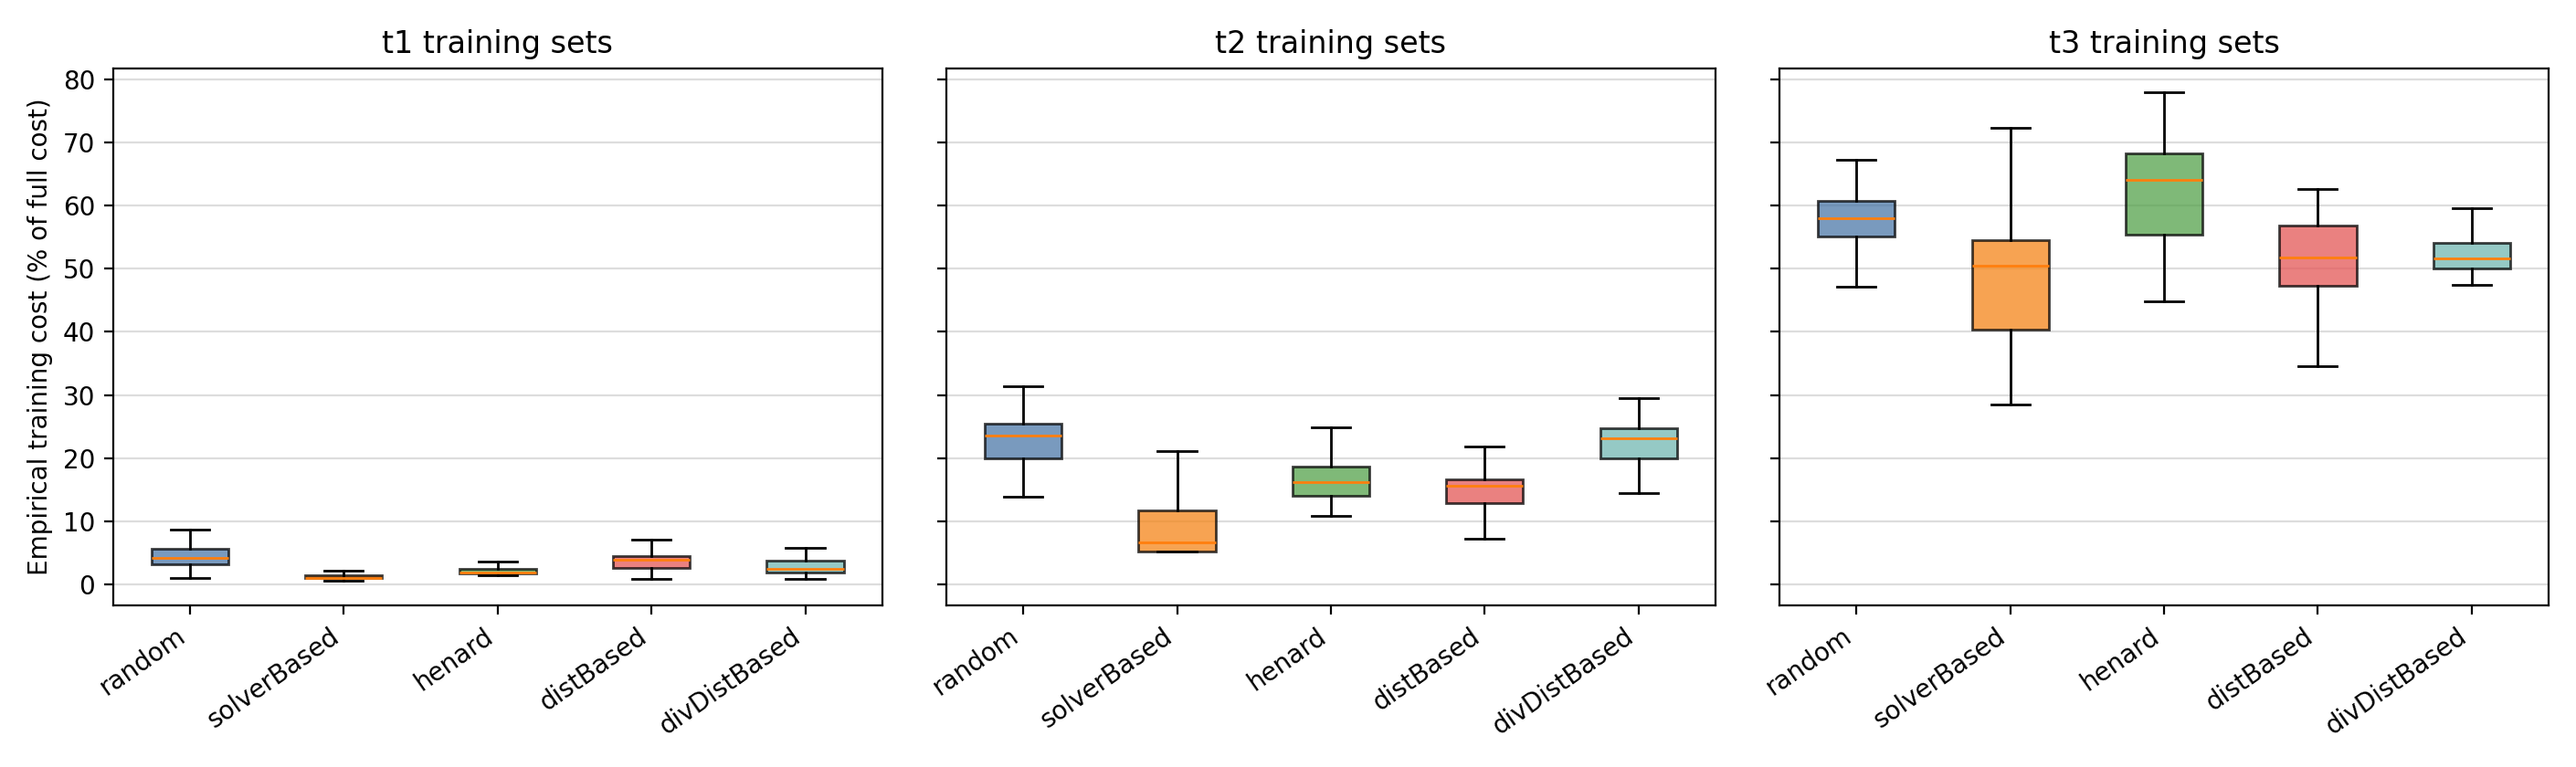
\includegraphics[width=\linewidth]{pic/results/lrzip_rq1_cost_distribution.png}
\caption{lrzip (adverse): heavy-tailed.}
\label{fig:rq1-vignette-lrzip}
\end{subfigure}\hfill
\begin{subfigure}{0.49\linewidth}
\centering
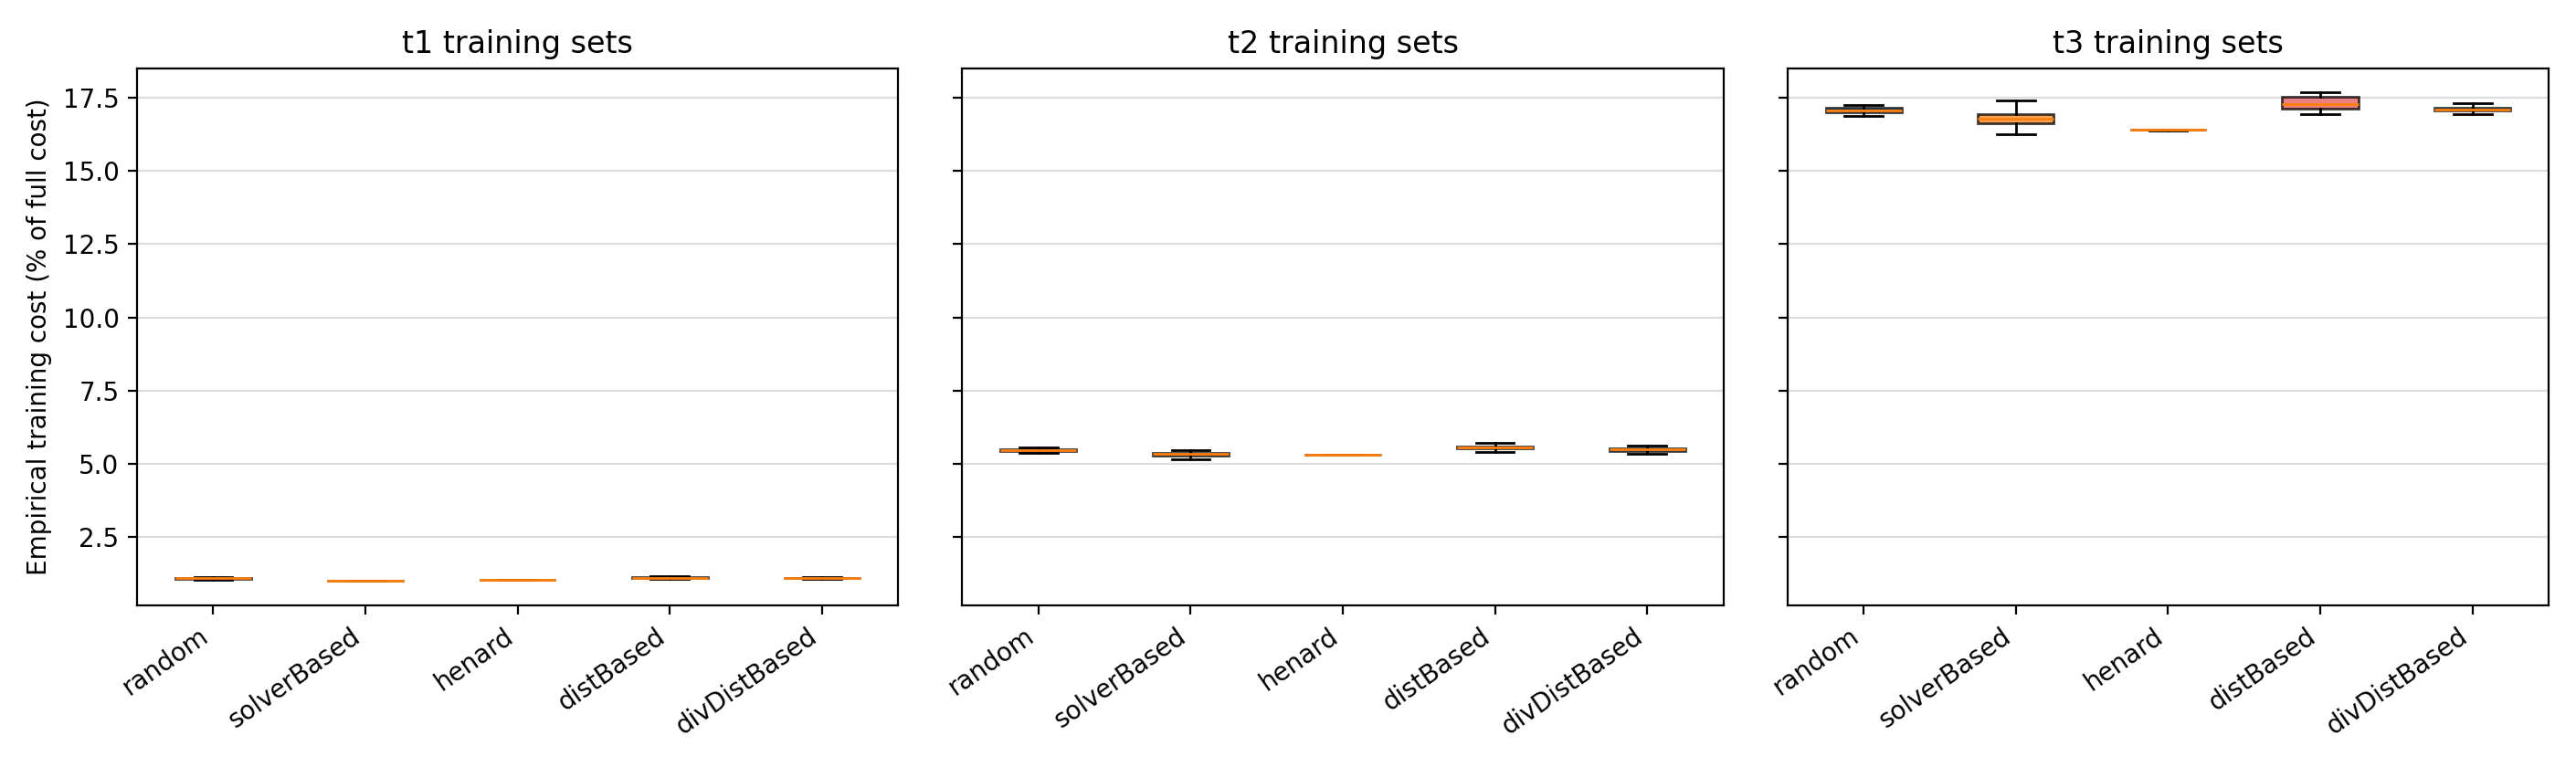
\includegraphics[width=\linewidth]{pic/results/llvm_rq1_cost_distribution.png}
\caption{LLVM (benign): tight.}
\label{fig:rq1-vignette-llvm}
\end{subfigure}
\caption{\StudyReplication RQ1 vignette --- cost distributions of the two
contrasting \StudyReplication extremes.}
\label{fig:rq1-vignettes}
\end{figure}

\paragraph*{\StudyEnergy.}
On \StudyEnergy (\Cref{tab:twins-summary}), per-configuration cost spans
almost three orders of magnitude across systems and cost properties,
from PostgreSQL\,11.2 (CV $0.058$ on energy --- the most homogeneous
case in the entire paper) to jump3r (CV $7.104$ on performance ---
the most heterogeneous). H1a is supported in $11/14$ system-cost
contexts and H1b in $14/14$. The two cost properties usually agree on
the qualitative direction but differ in magnitude (\eg jump3r:
performance CV $7.10$, energy CV $5.54$), confirming that the cost
\emph{dimension} matters and not only the cost \emph{level}.

\paragraph*{\StudyWorkload.}
The \dsWLI corpus ($9$ systems, $93$ workload contexts)
extends RQ1 to within-system workload variation. Cost CV at the
workload level ranges from $0.026$ (\texttt{dconvert} on the
\texttt{svg-large} workload) to $2.367$ (\texttt{kanzi} on the
\texttt{vmlinux} workload), with median $0.702$;
$p_{90}/p_{10}$ reaches $584$ on the same \texttt{kanzi/vmlinux}
context. Within a fixed system, workload alone can move the cost CV
by an order of magnitude
(\eg \texttt{lrzip}: $0.19$--$1.56$;
\texttt{kanzi}: $0.81$--$2.37$).
H1a pooled support across workloads is $0.86$
($I^{2}\!=\!0.59$, \Cref{tab:workload-impact-meta}); H1b is $0.88$
($I^{2}\!=\!0.41$). Both are mostly robust to workload, but
heterogeneity-magnitude is workload-sensitive within almost every
system.

\paragraph*{\StudyLinux.}
The \texttt{vmlinux} cost ranges from $1.17$\,MB to $1.78$\,GB on
v4.13, from $11.5$\,MB to $1.87$\,GB on v4.15, from $11.6$\,MB to
$1.96$\,GB on v5.0, and from $11.6$\,MB to $2.00$\,GB on v5.08
(\Cref{tab:linux-summary}). Cost CVs $1.43, 1.16, 1.16, 1.12, 1.08, 0.99, 1.01$ and
$p_{90}/p_{10}$ $4.61, 6.04, 5.80, 5.70, 5.21, 4.76, 4.02$ put all seven releases in the
``clearly heterogeneous'' regime, comparable to the worst \StudyReplication
systems. H1a is supported on all seven releases with the ``very
large'' magnitude label; H1b is supported with Kruskal--Wallis
$p<\!10^{-12}$ at every level on every release ($\eta^{2}$ up to
$0.41$). The H1 null is rejected on all seven.

\rqfinding{RQ1 take-away (cross-family).}{ Cost is far from uniform
\emph{wherever it is observable}. Per-configuration CV varies by
nearly three orders of magnitude across systems and cost dimensions
(PostgreSQL energy $0.058$ → jump3r performance $7.104$); within
the \dsWLI corpus, the same system across workloads varies
by an order of magnitude. At fixed $n$, strategy choice alone can
stretch training cost from $0.15\times$ to $1.6\times$ random on
\StudyReplication and to $\sim\!\!2\times$ random on Linux. The
equal-cost-per-configuration assumption is essentially correct on
LLVM and PostgreSQL\,11.2 only; everywhere else it fails, with a
wide quantitative range.}

\paragraph*{Hypothesis verdicts.}
\textbf{H1a} is supported on $6/7$ \StudyReplication systems
(LLVM is the only refutation), $22/34$ x264 cost-axis contexts (most
of the non-supports are cost-as-size axes with low CV),
$11/14$ \StudyEnergy contexts, $86\%$ pooled support across workload
contexts ($I^{2}\!=\!0.59$), and all seven \StudyLinux releases.
\textbf{H1b} is supported in every \StudyReplication scope ($7/7$), every x264
context ($34/34$), every \StudyEnergy context ($14/14$), $88\%$ pooled
across workload contexts ($I^{2}\!=\!0.41$), and all seven \StudyLinux
releases. The H1 null is rejected wherever cost is heterogeneous.

\subsection{RQ2 -- Sample Size as a Cost Proxy}
\label{subsec:results-rq2}

\paragraph*{\StudyReplication.}
\Cref{fig:rq2-calibration} compares $\mathit{SizePct}$ to
$\mathit{TrainCostPct}$ across \StudyReplication systems. Spearman correlation
is uniformly high ($\rho\in[0.879, 0.943]$); calibration drifts.

\begin{figure}[t]
\centering
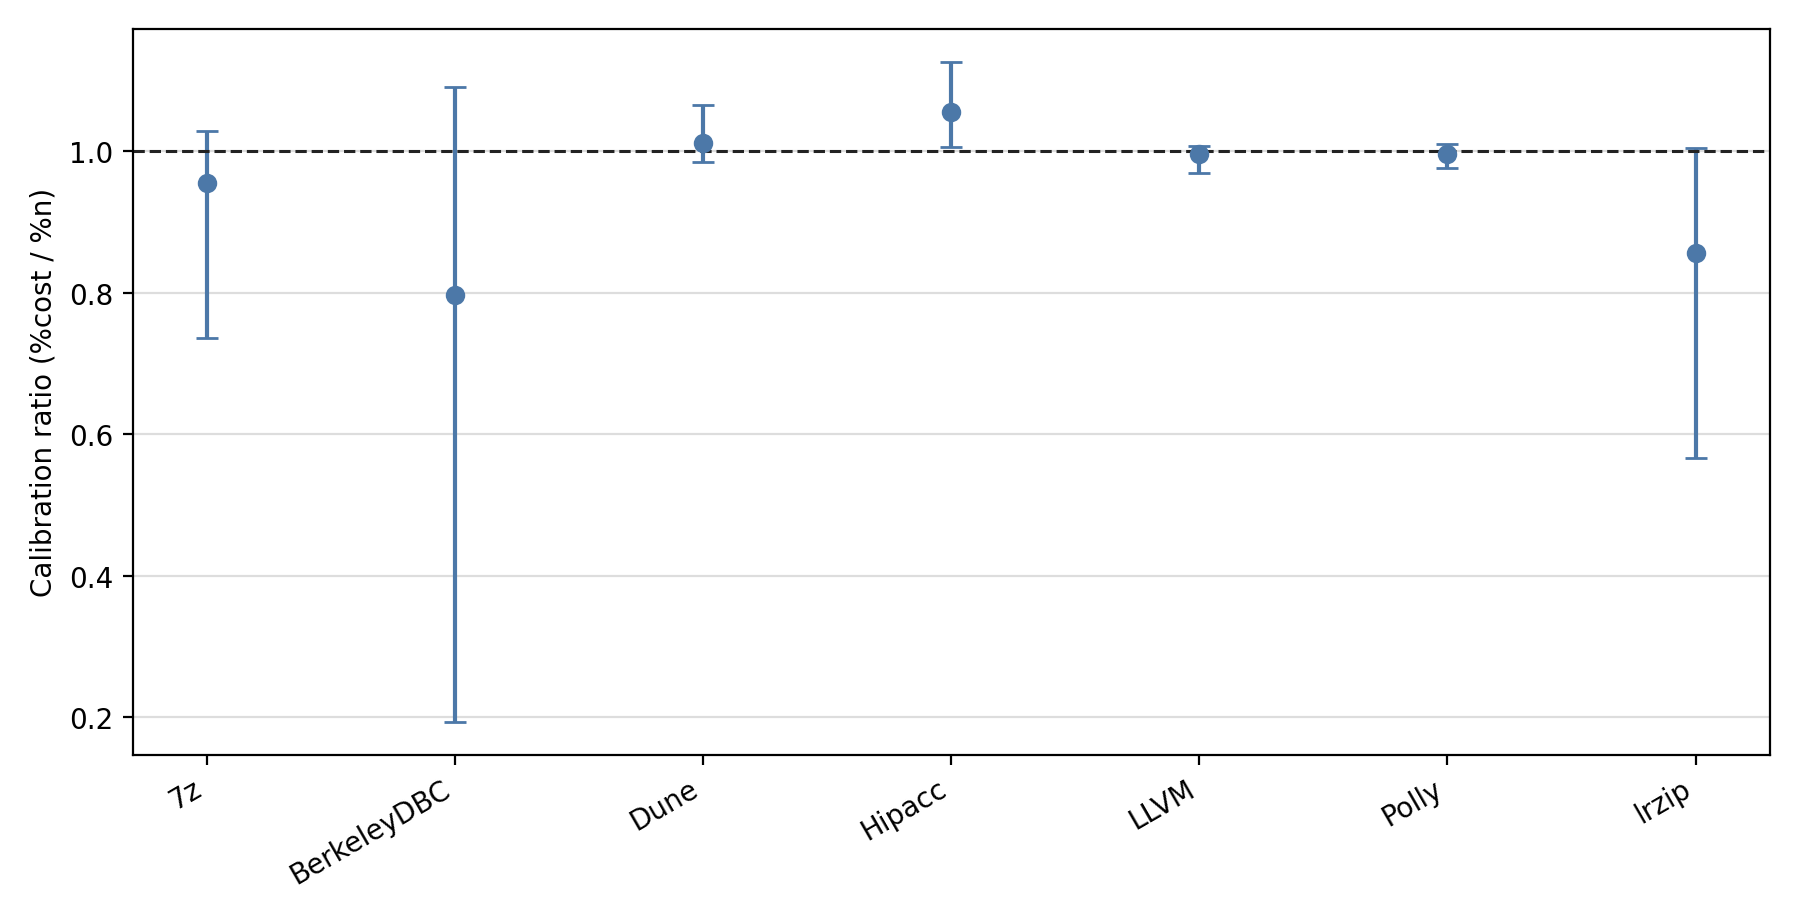
\includegraphics[width=\linewidth]{pic/results/fig_rq2_calibration_by_system.png}
\caption{\StudyReplication RQ2 --- calibration of $n$ as a cost proxy
across \StudyReplication systems.}
\label{fig:rq2-calibration}
\end{figure}

\emph{Adverse extreme -- BerkeleyDBC.} Median
$\mathit{TrainCostPct}/\mathit{SizePct}\!=\!0.797$: an $11\%$ sample
fraction buys $\sim\!\!8.8\%$ of the empirical cost on average, with
strategy-level IQR $[0.193, 1.091]$. The $\mathtt{henard\_t1}$
overhead reaches $0.155\times$ random on BerkeleyDBC, buying $84\%$
less wall-clock than the count budget would predict.

\emph{Benign extreme -- HIPAcc.} Median ratio $1.056$ with IQR
$[1.005, 1.126]$; $n$ is a usable cost budget within
$\sim\!\!13\%$.

\begin{figure}[t]
\centering
\begin{subfigure}{0.49\linewidth}
\centering
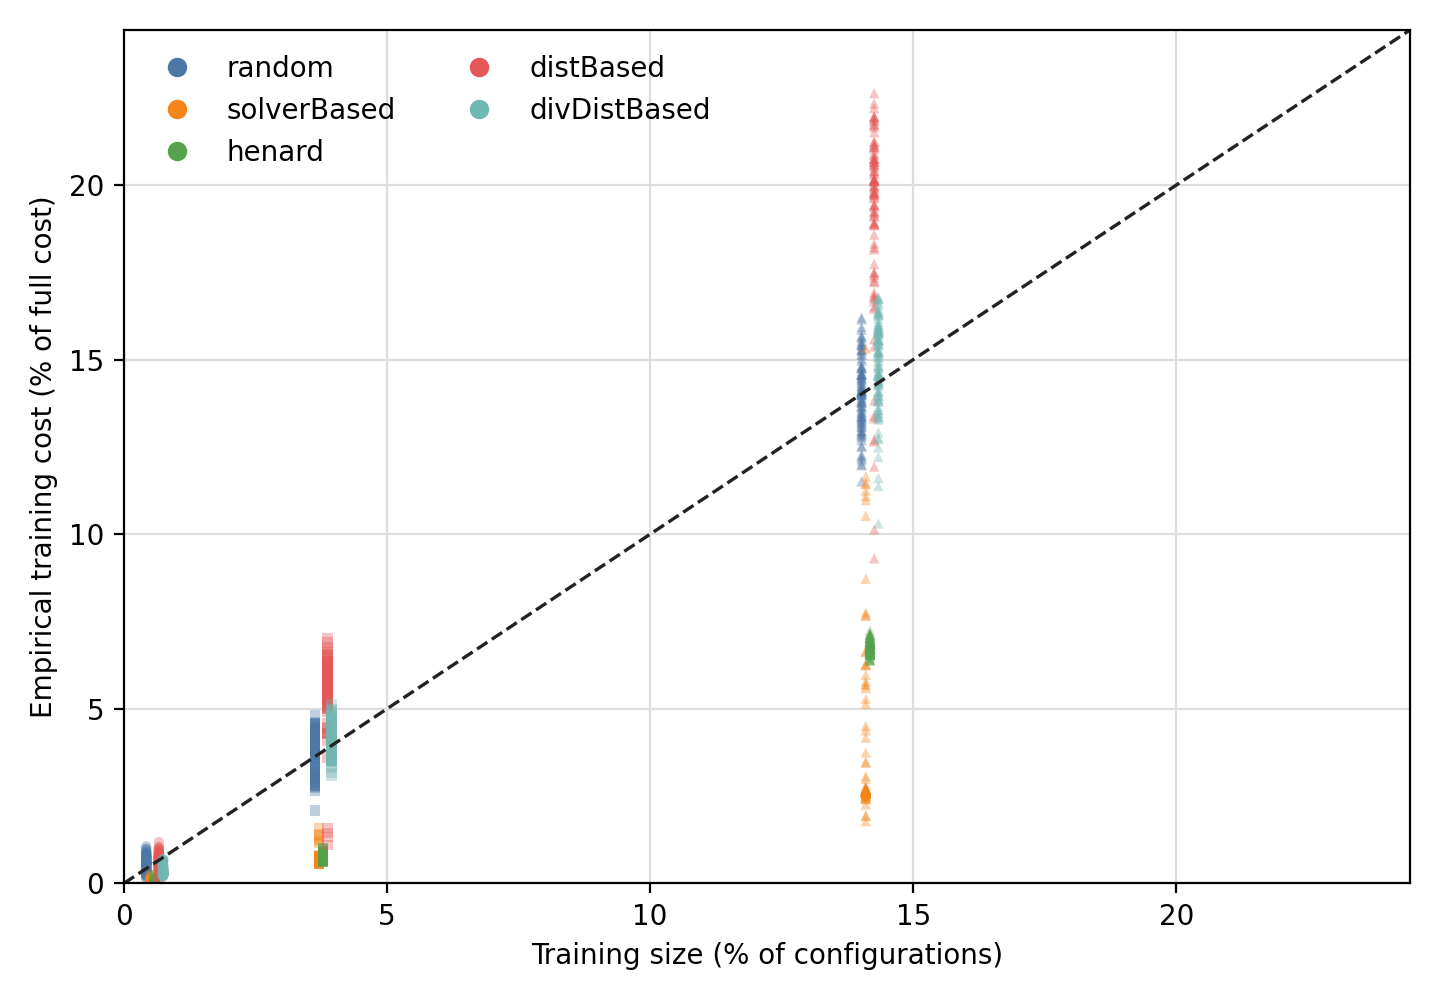
\includegraphics[width=\linewidth]{pic/results/bdbc_rq2_calibration.png}
\caption{BerkeleyDBC (adverse).}
\label{fig:rq2-vignette-bdbc}
\end{subfigure}\hfill
\begin{subfigure}{0.49\linewidth}
\centering
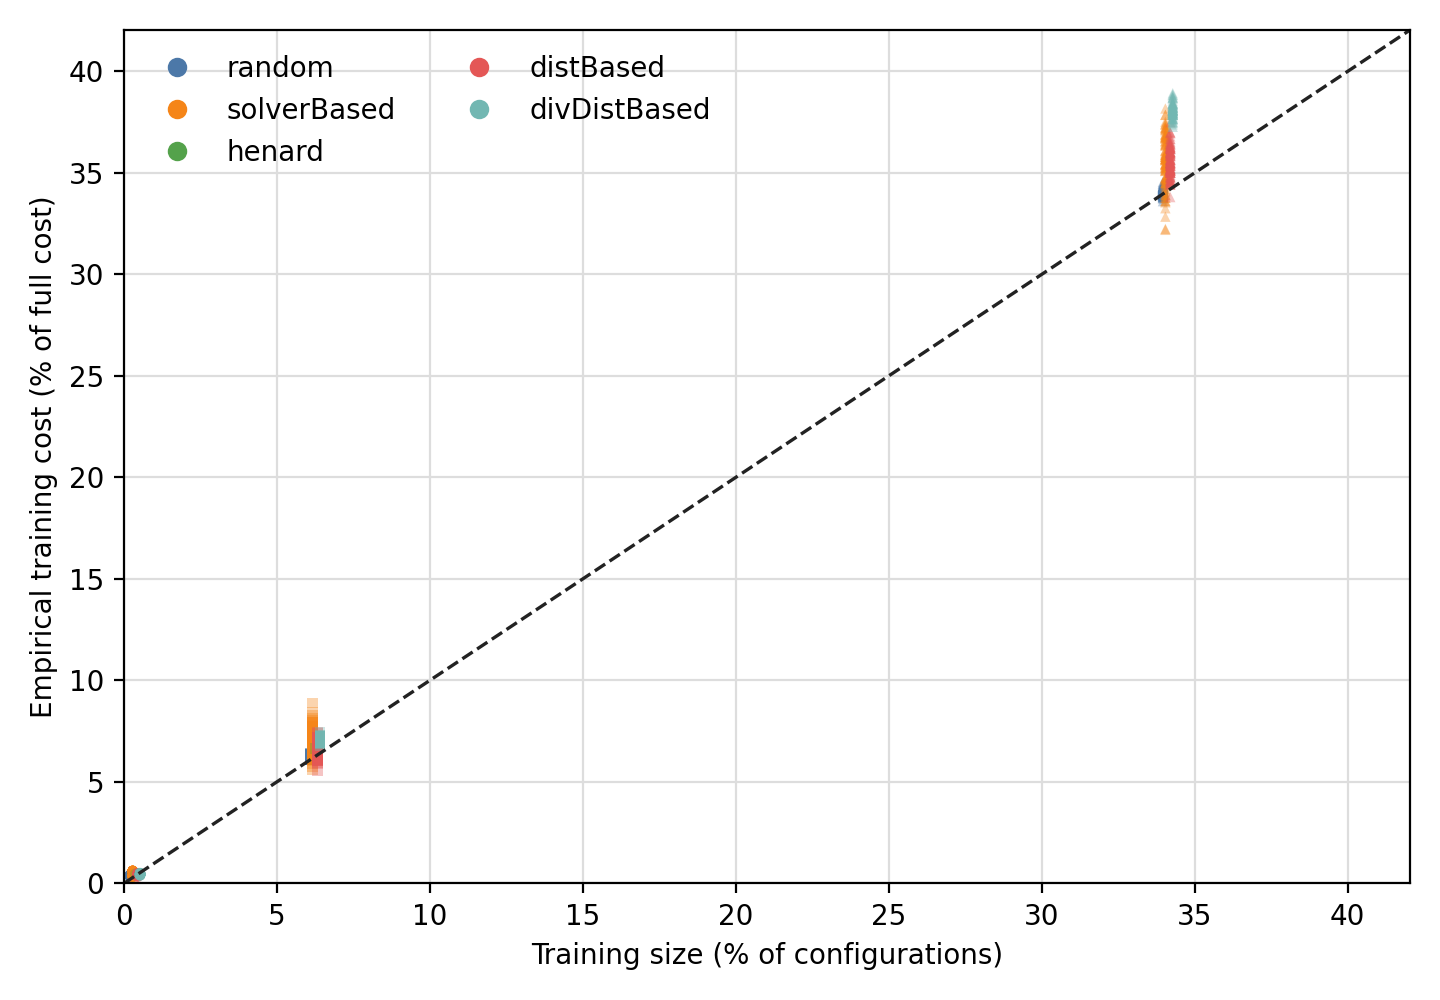
\includegraphics[width=\linewidth]{pic/results/hipacc_rq2_calibration.png}
\caption{HIPAcc (benign).}
\label{fig:rq2-vignette-hipacc}
\end{subfigure}
\caption{\StudyReplication RQ2 vignette ---
$\mathit{SizePct}$ vs $\mathit{TrainCostPct}$.}
\label{fig:rq2-vignettes}
\end{figure}

On x264, the per-input median calibration ratio sits within $\pm 2\%$
of $1$ in $32/34$ contexts, but per-strategy medians are biased:
$\mathtt{henard}$ at $0.75$ (cheap-favored under time-cost),
$\mathtt{twise}$ at $1.10$ (cost-biased). The bias is small in
aggregate but consistent in direction.

\paragraph*{\StudyEnergy.}
On \StudyEnergy, Spearman $\rho(n,\TrainCost)$ ranges from $0.710$ (lrzip,
performance-cost) to $0.996$ (PostgreSQL\,11.2): $n$ orders empirical
cost well in every system. Median calibration spans
$0.168$--$1.035$ across the $14$ system-cost contexts (the
$0.168$ on jump3r is the most extreme miscalibration in the paper).
\Cref{fig:twins-rq2-calibration} shows the per-system pattern.
\texttt{diversity} and \texttt{pairwise} are the strategies with the
most pronounced cost-side bias on this protocol; both favor extreme
combinations of options that correlate with the heavy tail of the
cost distribution on jump3r and brotli.

\begin{figure}[t]
\centering
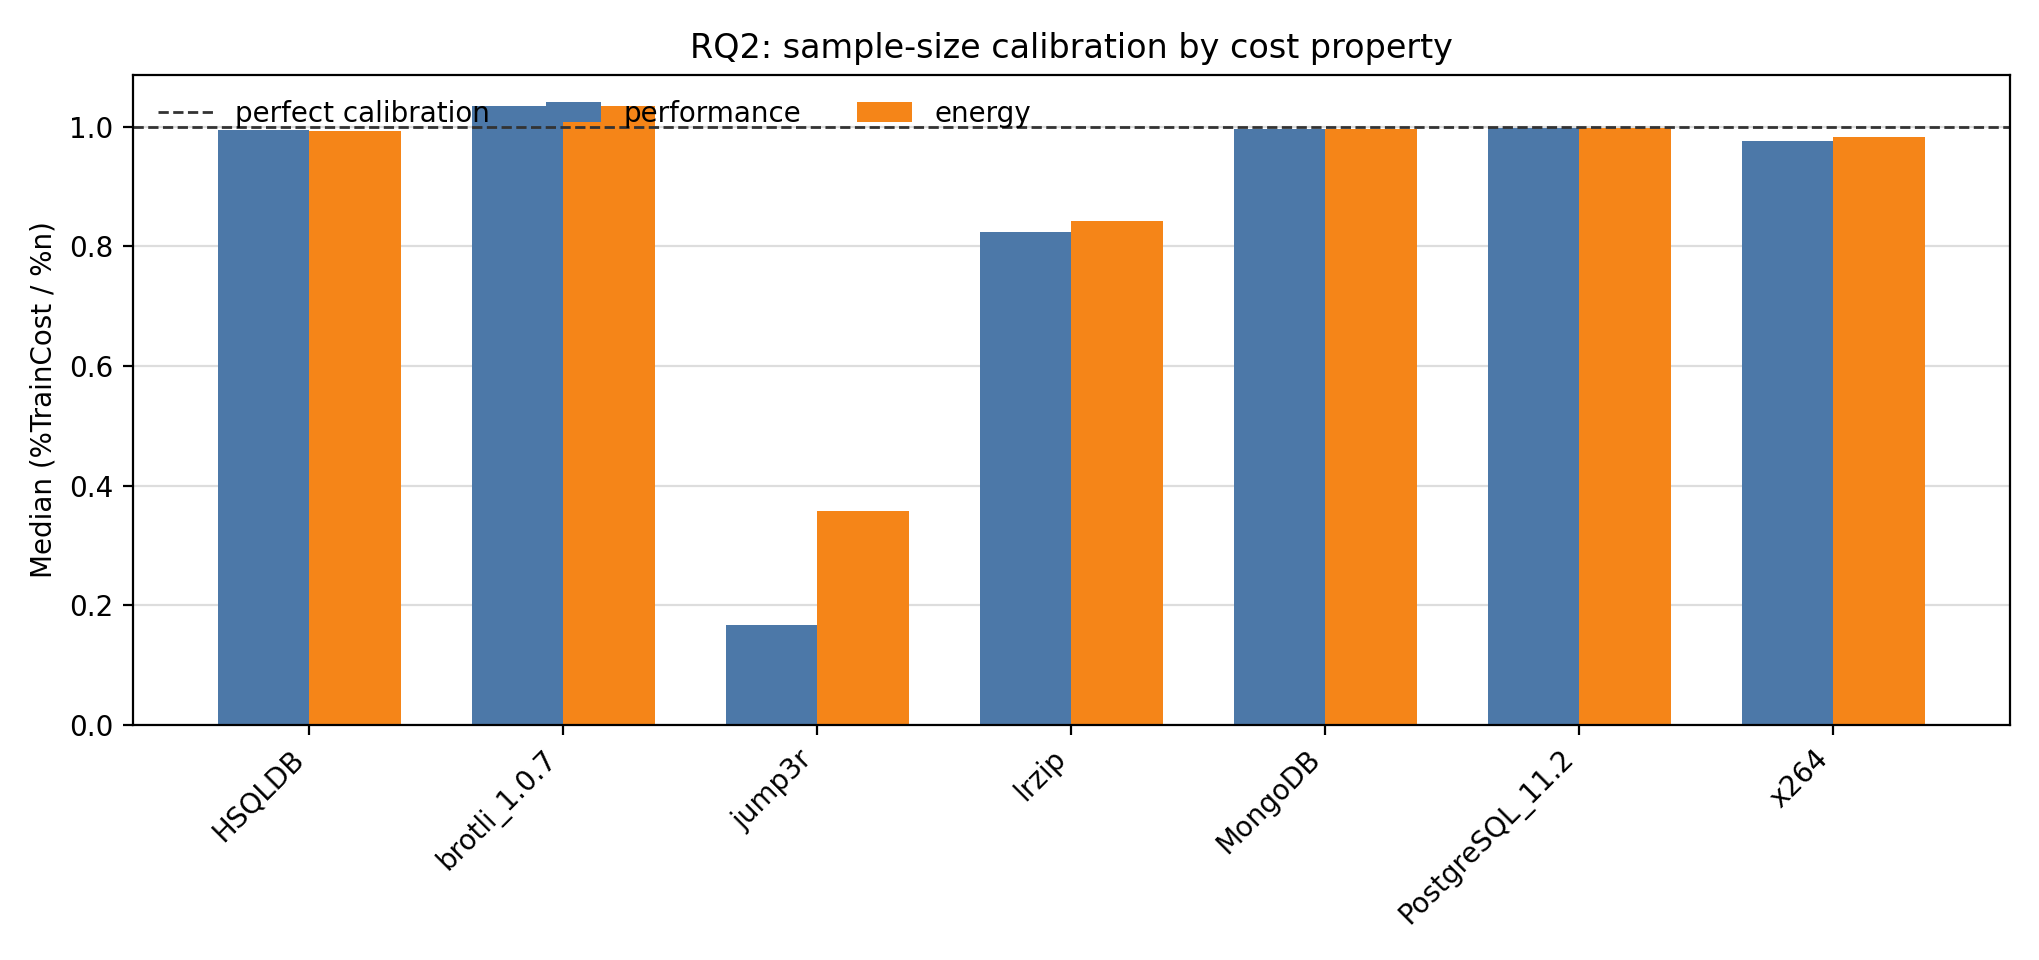
\includegraphics[width=\linewidth]{pic/results/twins_rq2_calibration.png}
\caption{\StudyEnergy RQ2 --- median calibration ratio by \StudyEnergy system and
cost property. PostgreSQL, MongoDB, HSQLDB, x264 hover near $1.0$;
brotli sits at $\sim\!\!1.03$; lrzip at $\sim\!\!0.83$; jump3r drops
to $0.17$--$0.36$.}
\label{fig:twins-rq2-calibration}
\end{figure}

\paragraph*{\StudyWorkload.}
H2a (rank correlation) is the most robust hypothesis of the paper:
pooled support $0.95$ across workloads with $I^{2}\!=\!0.00$
(\Cref{tab:workload-impact-meta}). Within a fixed system, $n$
remains rank-correlated with empirical cost on essentially every
workload. H2c (calibration depends on strategy) is also mostly
robust, pooled $0.90$ ($I^{2}\!=\!0.29$). H2b (median ratio not
centered at $1$) drops to $0.33$ pooled support with high
heterogeneity $I^{2}\!=\!0.76$: the workload often determines whether
the count proxy is miscalibrated enough to matter. The within-system
median ratio range is
$0.661$--$1.059$ across $93$ contexts.

\paragraph*{\StudyLinux.}
\Cref{fig:linux-rq2-vignettes} shows the per-strategy
$\mathit{TrainCostPct}$ vs $\mathit{SizePct}$ scatter on v4.13 and
v5.08. Three calibration regimes replicate four times across the
Linux quartet:
\begin{itemize}
    \item \emph{Calibrated:} \texttt{random}, \texttt{balanced},
    \texttt{coverage} -- median ratios within $\pm 2.6\%$ of $1$ on
    every release; the strongest robust null in the study.
    \item \emph{Strong upward drift:} \texttt{diversity} reaches
    $2.28, 2.23, 2.27, 2.06, 2.09, 2.00, 2.02$ (window $[2.00, 2.28]$) across v4.13, v4.15, v4.20, v5.0, v5.04, v5.07, v5.08 ---
    seven independent randconfig pools, magnitudes within $\pm 15\%$
    of one another. Mechanism: farthest-first in Hamming distance
    picks high-option-count configurations, which on randconfig
    pools are systematically the larger kernels.
    \item \emph{$n$-dependent drift:} \texttt{uncertainty}'s
    aggregate ratio is direction-stable but pool-dependent
    ($1.246, 0.996, 0.943, 0.979, 0.878, 0.839, 0.946$); aligned by absolute $n$, the
    pattern is unanimous --- AL drifts toward cheap at small $n$
    and toward expensive at large $n$ on every release.
\end{itemize}
The cross-version Linux seam is the key insight: a single-pool view
of \texttt{uncertainty} would land on a misleading aggregate verdict
($+25\%$ on v4.13 alone, $-5\%$ on v5.08 alone); only the
multi-pool view reveals that AL is direction-sensitive to $n$ with a
pool-dependent cross-over.

\begin{figure}[t]
\centering
\begin{subfigure}{0.49\linewidth}
\centering
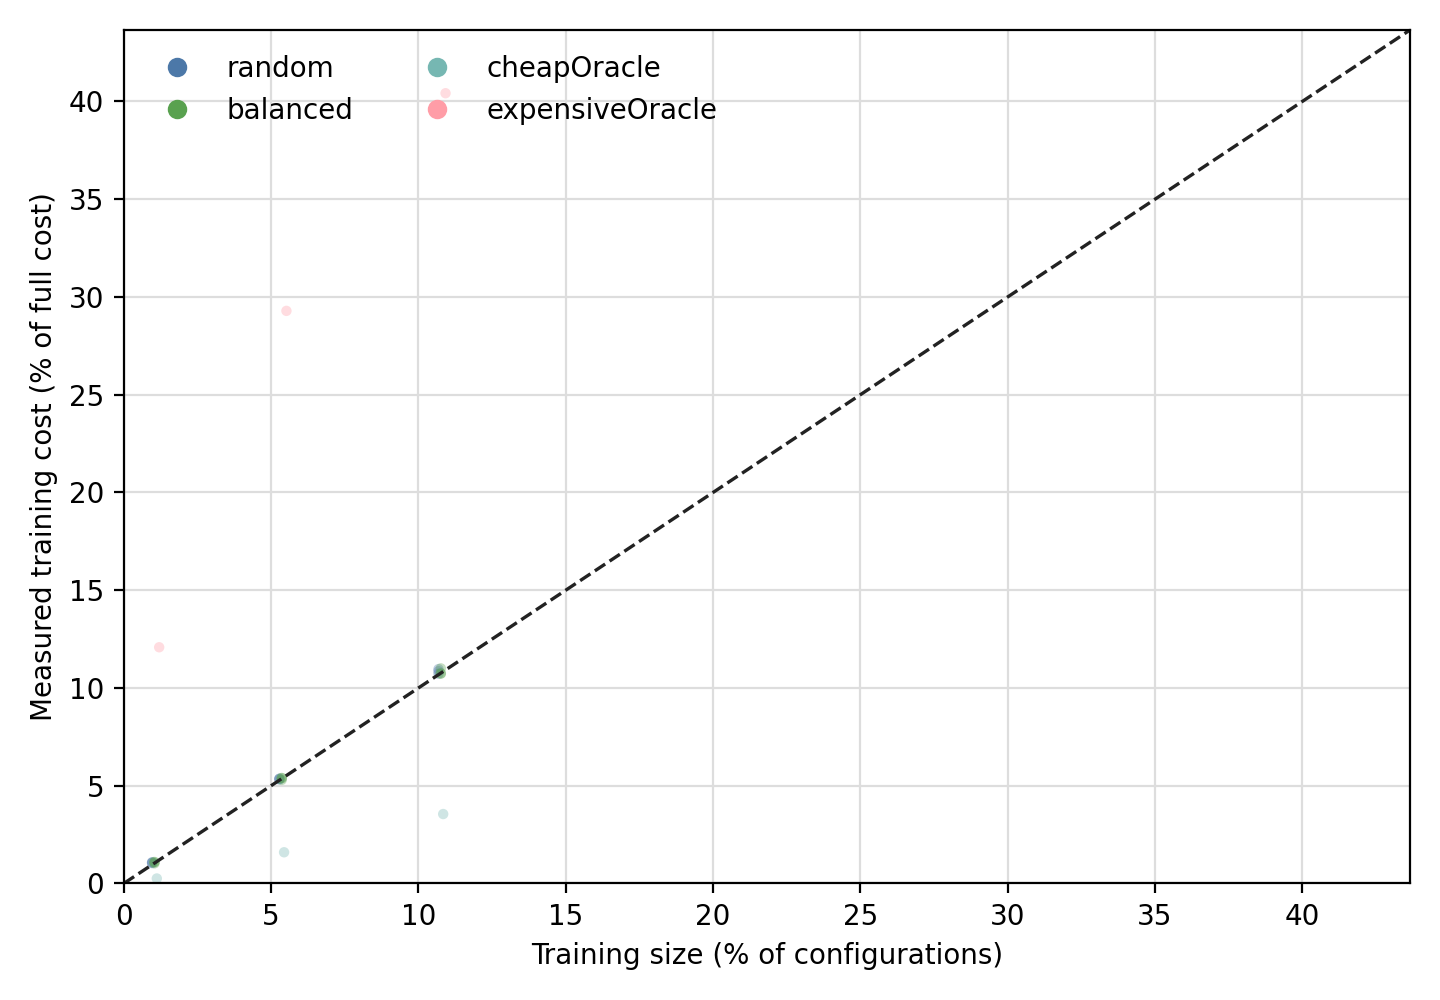
\includegraphics[width=\linewidth]{pic/results/linux413_rq2_calibration.png}
\caption{Linux v4.13.}
\label{fig:linux413-rq2}
\end{subfigure}\hfill
\begin{subfigure}{0.49\linewidth}
\centering
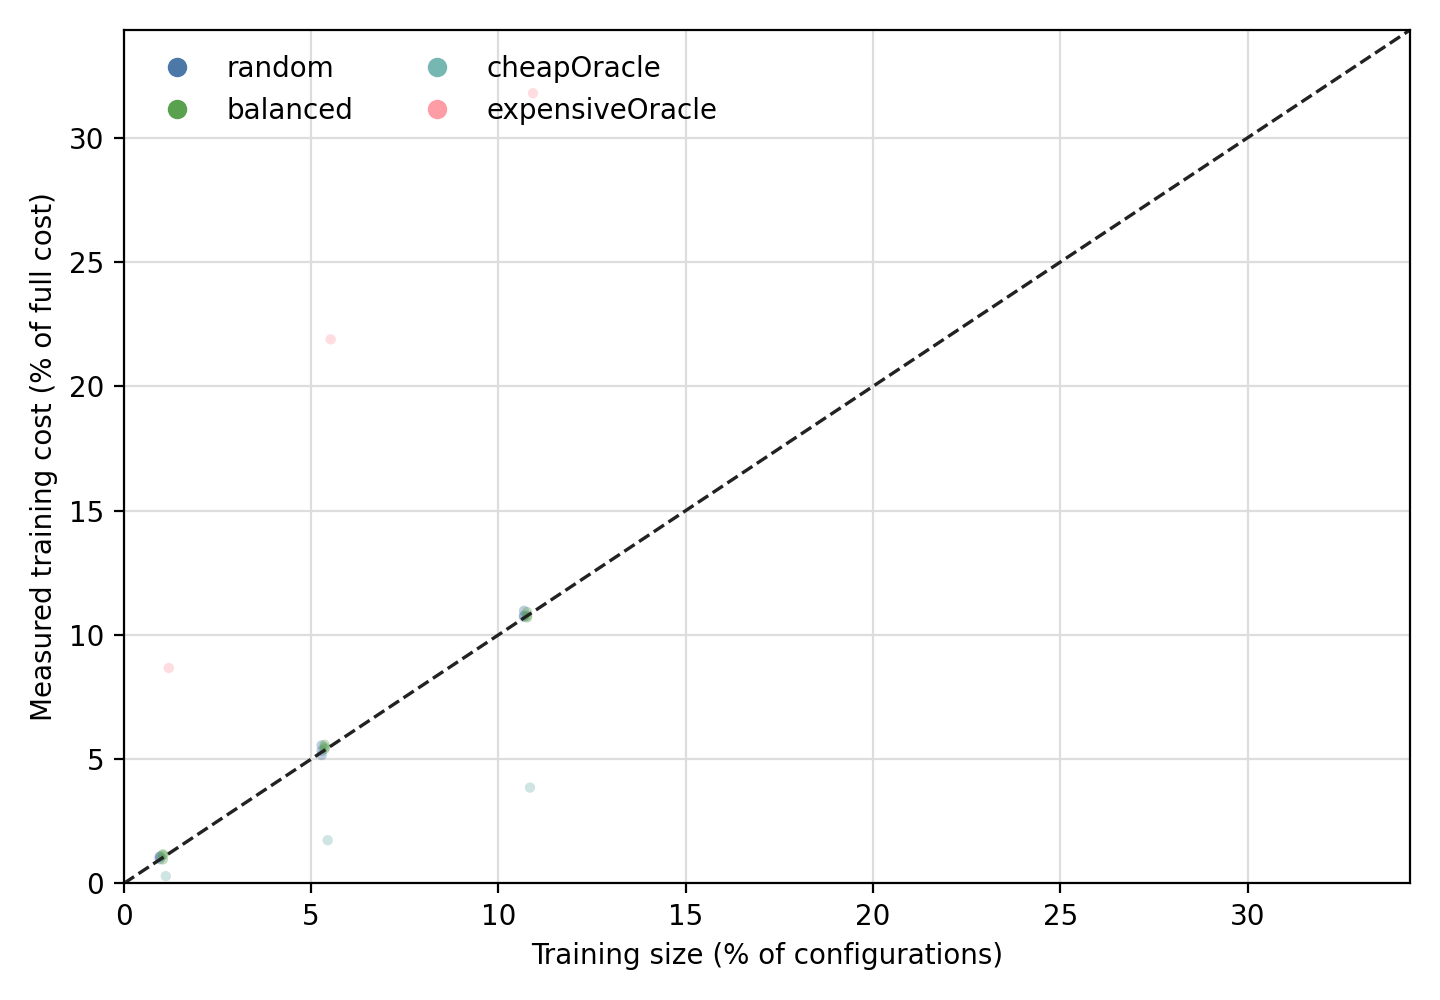
\includegraphics[width=\linewidth]{pic/results/linux508_rq2_calibration.png}
\caption{Linux v5.08.}
\label{fig:linux508-rq2}
\end{subfigure}
\caption{\StudyLinux RQ2 --- $\mathit{SizePct}$ vs $\mathit{TrainCostPct}$
per strategy. \texttt{diversity} drifts to $\sim\!\!2\times$ on both;
\texttt{uncertainty} drifts upward at large $n$ on both, but
\emph{downward} at small $n$ on v5.08.}
\label{fig:linux-rq2-vignettes}
\end{figure}

\rqfinding{RQ2 take-away (cross-family).}{ $n$ is correlated with
empirical cost on \emph{every} system in \emph{every} family
($\rho\geq 0.71$ everywhere; H2a is the most robust hypothesis of
the paper, pooled support $0.95$ on workload contexts with
$I^{2}\!=\!0.00$). Calibration is not. Median calibration drifts to
$0.80$ on BerkeleyDBC (\StudyReplication), $0.17$ on jump3r (\StudyEnergy); the
workload alone can shift the verdict on H2b ($I^{2}\!=\!0.76$); on
Linux, four of seven calibration regimes replicate but the verdict
is strategy-conditional, not system-wide. $n$ is a useful coarse
ordering of cost; it is not a substitute for measured cost.}

\paragraph*{Hypothesis verdicts.}
\textbf{H2a} is supported in every scope: $7/7$ \StudyReplication,
$34/34$ x264, $14/14$ \StudyEnergy, pooled $0.95$ across workloads
($I^{2}\!=\!0.00$), all seven \StudyLinux releases ($\rho\in[0.966, 0.968]$ across the seven).
\textbf{H2b} is supported on the three \StudyReplication systems where the
practical bias exceeds $5\%$ (BerkeleyDBC $0.797$, lrzip $0.856$,
HIPAcc $1.056$); inconclusive on the others; on x264 supported in
$2/34$ contexts; on \StudyEnergy $4/14$; pooled $0.33$ on workloads with
$I^{2}\!=\!0.76$ (workload-sensitive); on Linux refuted at the
aggregate level on every release but the per-strategy decomposition
flags \texttt{diversity} as miscalibrated on all seven.
\textbf{H2c} is supported in every scope: $7/7$ \StudyReplication, $34/34$
x264 ($\eta^{2}$ up to $0.74$), $14/14$ \StudyEnergy, pooled $0.90$
($I^{2}\!=\!0.29$) across workloads, all seven \StudyLinux releases
($\eta^{2}\!\in\![0.10, 0.33]$ on the seven releases).

\subsection{RQ3 -- Robustness of Conclusions to the Cost Model}
\label{subsec:results-rq3}

\paragraph*{\StudyReplication.}
\Cref{fig:rq3-rq4-decision} reports rank flips and Pareto Jaccard
between count-cost and empirical-cost objectives, swept over
$\lambda\in\{0.1,0.25,0.5,1,2,4,10\}$. The picture splits into three
\StudyReplication regimes:
\begin{itemize}
    \item \textbf{Stable} (Dune, HIPAcc, LLVM, Polly): $0/7$ rank
    flips, Kendall $\tau\geq 0.94$. The cost-model choice does not
    change the top recommendation.
    \item \textbf{Marginal} (7Z, BerkeleyDBC): $1/7$ flips, $\tau$
    $0.60$--$0.83$.
    \item \textbf{Unstable} (lrzip): $5/7$ flips, $\tau\!=\!0.80$.
    The recommended top-$1$ strategy changes for the majority of
    cost budgets.
\end{itemize}
Cross-system, the heterogeneity-predicts-fragility correlation H3b
holds: Spearman $\rho(\mathrm{CV}, \text{flips})\!=\!0.90$,
$p\!=\!6.3\!\times\!10^{-3}$ on the $7$ \StudyReplication systems.

\begin{figure}[t]
\centering
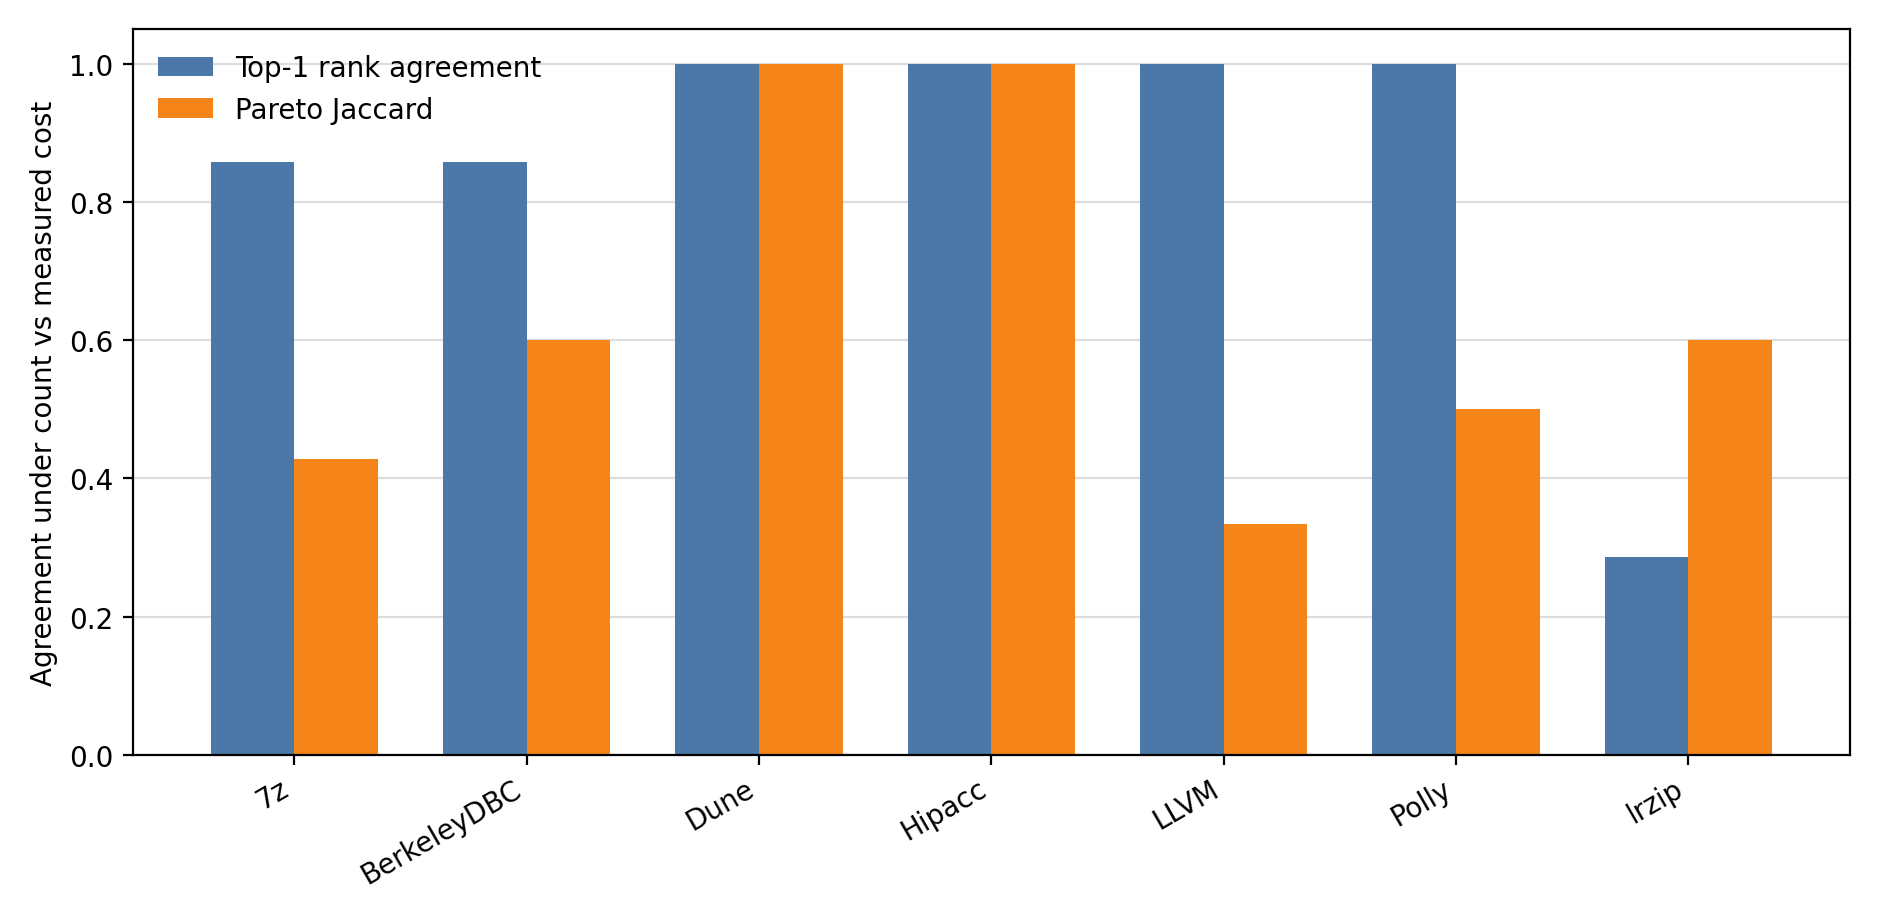
\includegraphics[width=\linewidth]{pic/results/fig_rq3_rq4_decision_change_by_system.png}
\caption{\StudyReplication RQ3/RQ4 --- decision-level consequences across
\StudyReplication systems.}
\label{fig:rq3-rq4-decision}
\end{figure}

\emph{Adverse extreme -- lrzip.} $5/7$ values of $\lambda$ produce
a different top-$1$ recommendation; the empirical-cost frontier admits a
different mix of best simple pairs than the count-cost frontier.

\emph{Benign extreme -- LLVM.} $0/7$ flips,
$\tau\!=\!0.945$, top-$3$ overlap $1.0$ at every $\lambda$.

\begin{figure}[t]
\centering
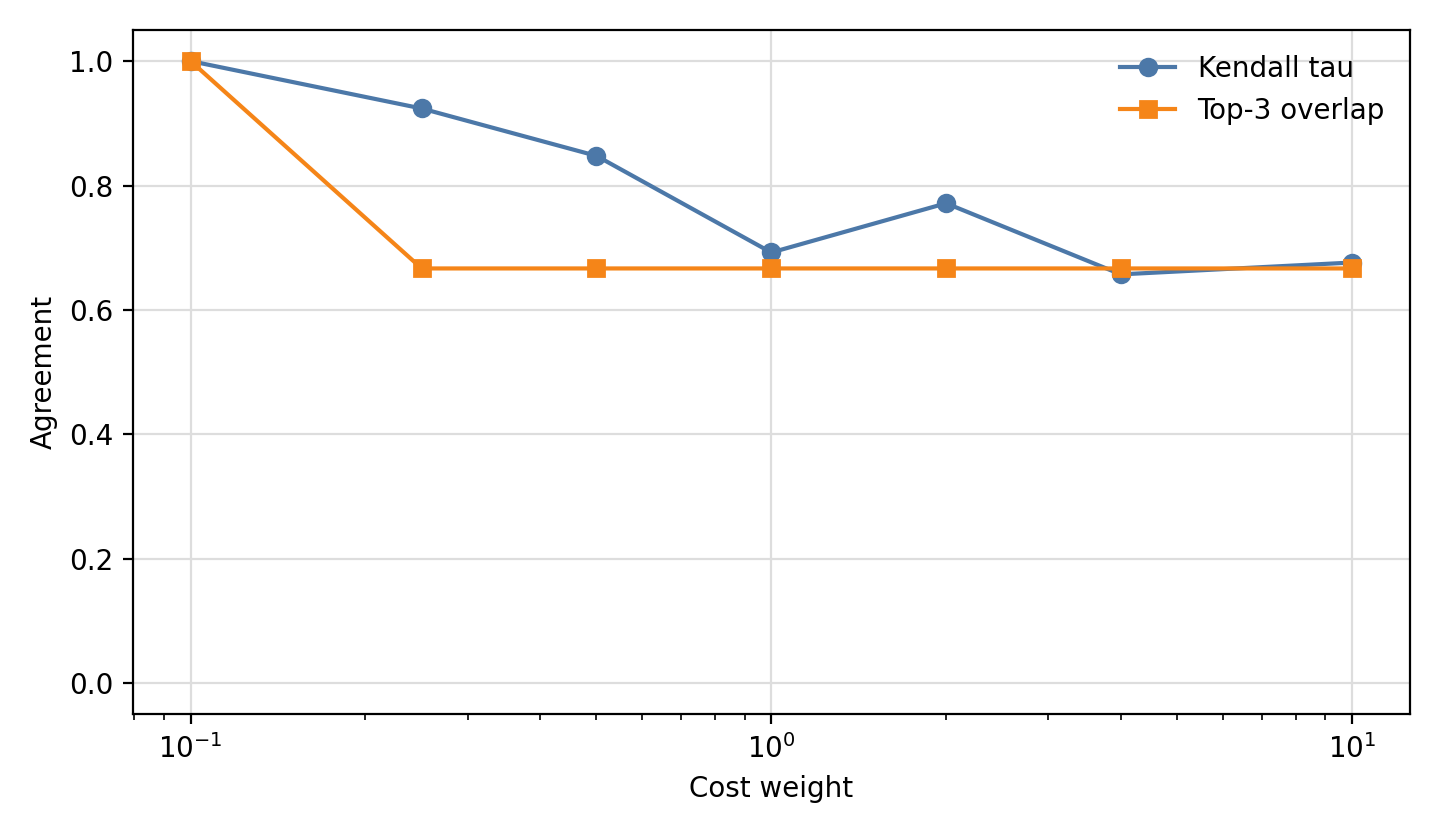
\includegraphics[width=0.95\linewidth]{pic/results/lrzip_rq3_rank_stability.png}
\caption{\StudyReplication RQ3 vignette --- lrzip rank stability across
$\lambda$.}
\label{fig:rq3-vignette-lrzip}
\end{figure}

On x264, top-$1$ agreement varies with the scenario
(\Cref{fig:rq3-x264-scenarios}, \Cref{tab:x264-matrix-summary}):
$0.95$ for $(\text{cost}\!=\!\text{time}, \text{target}\!=\!\text{time})$,
down to $0.82$ for the asymmetric
$(\text{cost}\!=\!\text{time}, \text{target}\!=\!\text{size})$
scenario --- predicting size while paying time-based cost flips the
top-$1$ recommendation in $21/119$ $(\text{input},\lambda)$ cases,
more than three times as often as the symmetric scenario.

\begin{figure}[t]
\centering
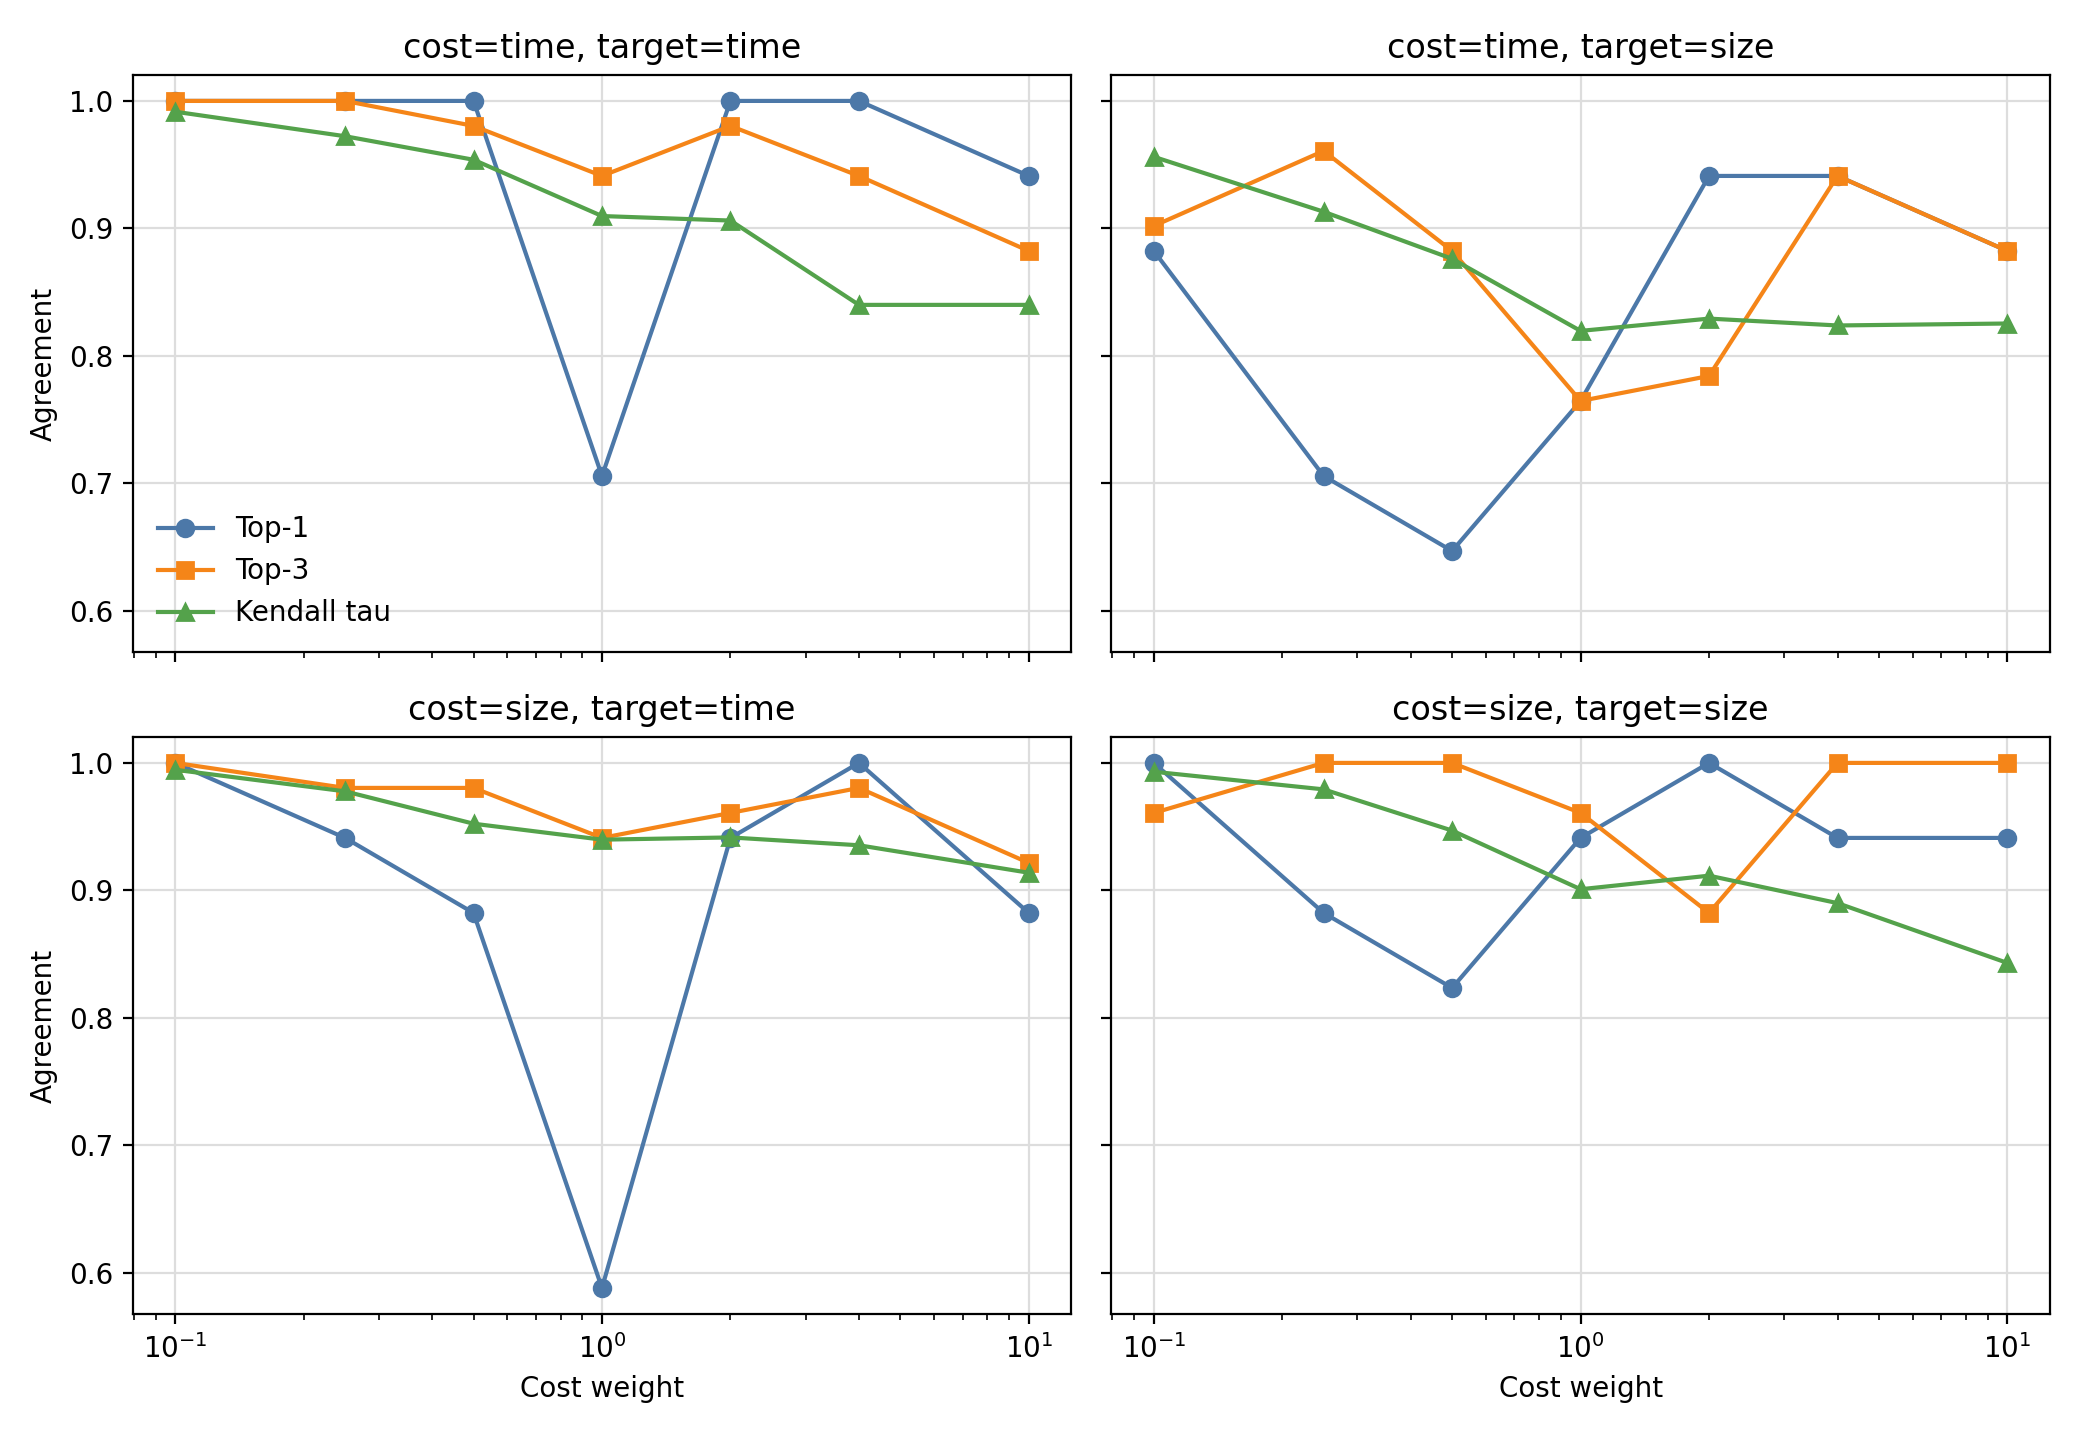
\includegraphics[width=\linewidth]{pic/results/fig_rq3_rank_agreement_by_scenario.png}
\caption{\StudyReplication RQ3 (x264) --- rank agreement across the four
cost--target scenarios.}
\label{fig:rq3-x264-scenarios}
\end{figure}

\paragraph*{\StudyEnergy.}
On \StudyEnergy, top-$1$ rankings differ in $24/28$ scenarios.
\Cref{fig:twins-rq3-heatmap} shows the agreement matrix; the four
scenarios that agree at every $\lambda$ are the calibrated PostgreSQL
cases. The least-stable scenarios are on \texttt{brotli\,1.0.7}:
\emph{three} of its four scenarios reach top-$1$ agreement of zero
(every $\lambda$ flips). \texttt{jump3r} exhibits the same pattern in
two of four scenarios. The dark cells on brotli and jump3r are the
visual signature of a generated-sampling protocol on a heavy-tailed
cost distribution.

\begin{figure}[t]
\centering
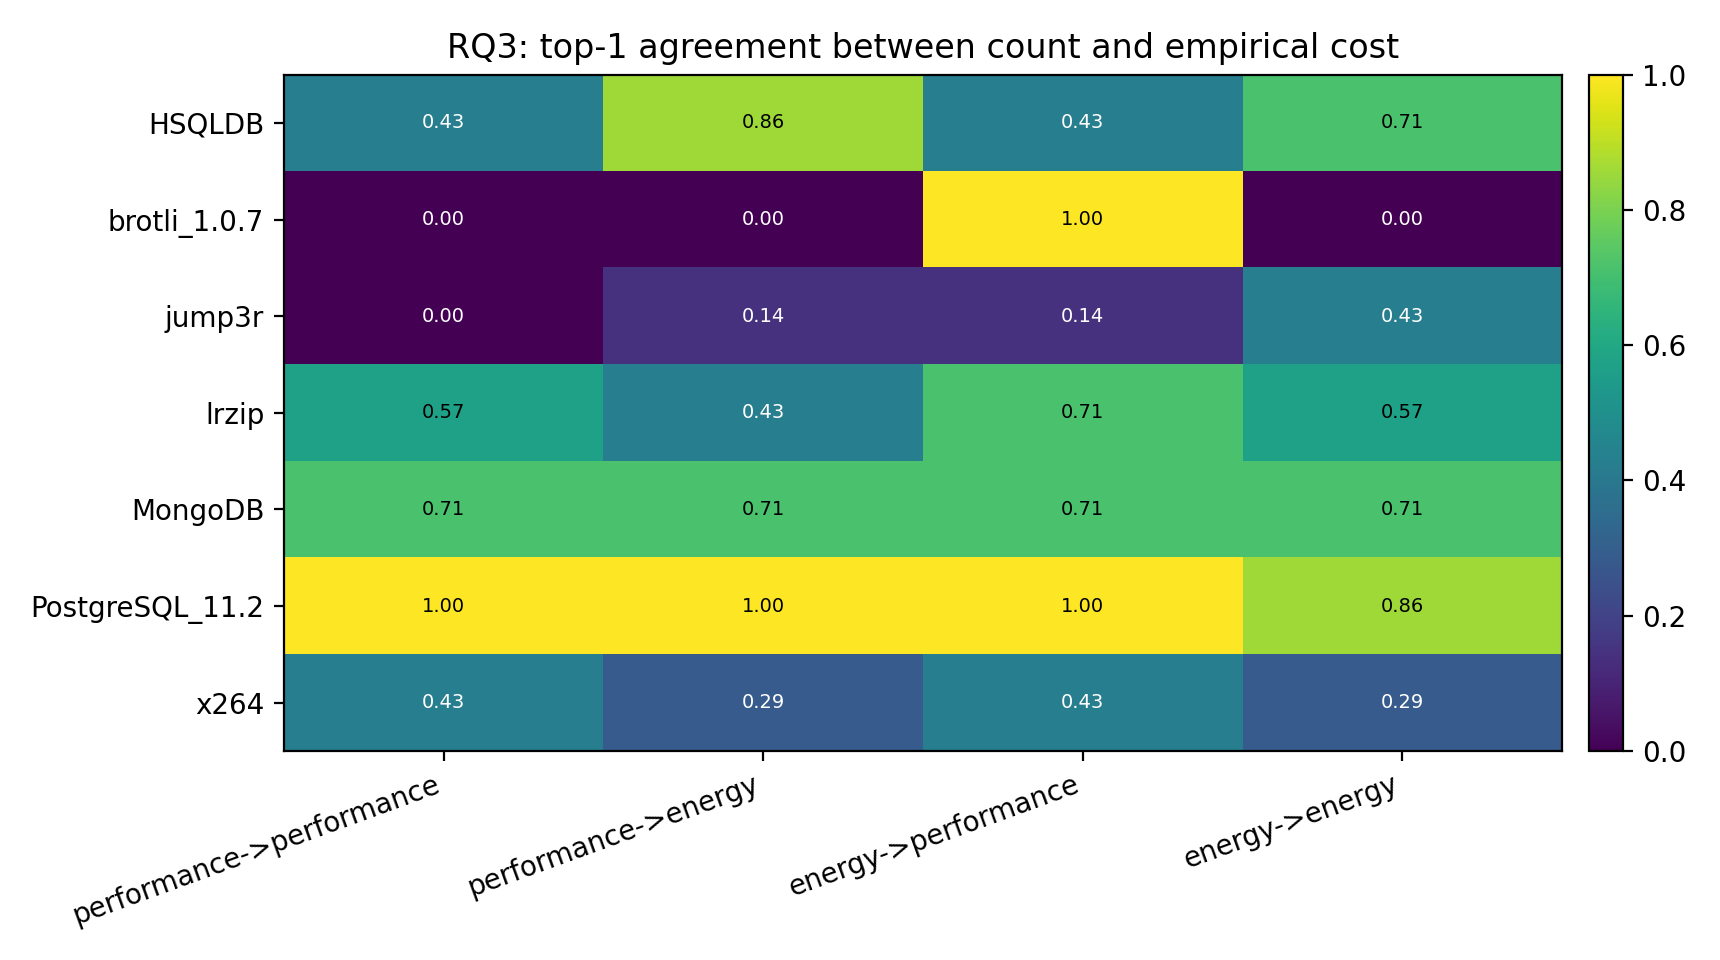
\includegraphics[width=\linewidth]{pic/results/twins_rq3_heatmap.png}
\caption{\StudyEnergy RQ3 --- top-$1$ rank agreement heatmap (Twins
system $\times$ cost-target scenario).}
\label{fig:twins-rq3-heatmap}
\end{figure}

\paragraph*{\StudyWorkload.}
H3a pooled support is $0.80$ across the $93$ workload contexts with
high heterogeneity $I^{2}\!=\!0.69$. The within-system extremes are
informative: \texttt{xz} supports H3a on $13/13$ workloads (every
workload exhibits at least one rank flip), while \texttt{lrzip}
supports it on only $2/13$ workloads (most workloads stable).
\texttt{kanzi} is intermediate: count-based and empirical Pareto
frontiers differ on only $3/9$ workloads despite strong cost
heterogeneity. Workload variance accounts for about $55\%$ of the
within-system residual in top-$1$ agreement (versus $22\%$ for mean
Kendall $\tau$). Once a system is fixed, the workload still
materially changes the probability of recommending a different
sampling strategy.

\paragraph*{\StudyLinux.}
Top-$1$ rank flips between count-cost and empirical-cost objectives
hit $2/7$ on v4.13, v4.15, v5.0, and $6/7$ on v5.08
(\Cref{tab:linux-summary}). The cluster of three at $2/7$ spans
pool sizes $19{,}952$ to $92{,}562$ and cost CVs $1.12$ to $1.43$,
so neither pool size nor cost CV explains v5.08's $6/7$. The
proximate cause is v5.08's specific level grid landing on tied
absolute $n$'s where MRE differences are sub-threshold; the
empirical-cost ranking is more discriminative than the count
ranking, and surfaces as a flip whenever the level grid produces
ties. \emph{The H3b heterogeneity-predicts-fragility correlation
observed on \StudyReplication ($\rho\!=\!+0.90$) does not extend to the Linux
pool}: with four of seven flip counts tied at $2$, the cross-Linux
$\rho(\mathrm{CV}, \text{flips})$ is dominated by the v5.08 outlier
and there is no monotone trend. This is a protocol effect, not a
heterogeneity effect, and the load-bearing reason we report Linux
separately rather than aggregating it with \StudyReplication into a joint H3b
correlation.

\rqfinding{RQ3 take-away (cross-family).}{ Rankings sometimes flip,
sometimes don't, and the failure mode is family-dependent. On
\StudyReplication, heterogeneity predicts fragility ($\rho\!=\!0.90$,
$\rho\geq 5$ flips on lrzip; $0$ flips on LLVM/Polly/Dune/HIPAcc).
On \StudyEnergy, heavy-tailed \StudyEnergy systems (jump3r, brotli, lrzip) reach
top-$1$ agreement of $0$ on multiple scenarios. On \StudyWorkload, the
workload itself moves the verdict on $\sim\!\!55\%$ of within-system
variance. On \StudyLinux, three of seven releases share the same $2/7$
flip count while v5.04 flips $7/7$, v5.07 flips $4/7$, and v5.08 flips $6/7$ for level-grid reasons rather
than heterogeneity reasons, contradicting the cross-system H3b
pattern. The cost-model choice is not a cosmetic detail in any
family.}

\paragraph*{Hypothesis verdicts.}
\textbf{H3a} is the existential claim of the paper: supported in
$3/7$ \StudyReplication systems and $25/68$ x264 input/scenario pairs, in
$24/28$ \StudyEnergy scenarios, $80\%$ pooled support across workload
contexts ($I^{2}\!=\!0.69$), and on all seven \StudyLinux releases.
\textbf{H3b} is supported on the cross-system \StudyReplication correlation
($\rho\!=\!0.90$, $p\!=\!6.3\!\times\!10^{-3}$), supported on \StudyEnergy
(heavy-tailed systems flip more), but \emph{refuted} on Linux: three
of seven \StudyLinux releases share the same flip count across a $5\times$
pool-size range and a $1.27\times$ CV range. The H3b correlation is
within-family, not cross-family.

\subsection{RQ4 -- Pareto Efficiency under Empirical Cost}
\label{subsec:results-rq4}

\paragraph*{\StudyReplication.}
The Pareto Jaccard panel of \Cref{fig:rq3-rq4-decision} ranges from
$0.33$ (LLVM) to $1.00$ (Dune, HIPAcc) on \StudyReplication. The empirical-cost
view \emph{systematically reveals more} non-dominated $(s,n)$ pairs
than the count view: $9$ vs $3$ on LLVM, $7$ vs $3$ on 7Z, $6$ vs
$3$ on Polly, $5$ vs $3$ on BerkeleyDBC and lrzip. Size-based
recommendations over-prune the choice space.

\emph{Adverse extreme -- LLVM (Jaccard $0.33$, lowest).} LLVM has
the lowest cost CV ($0.072$) and the lowest Pareto Jaccard, which
looks paradoxical: under count-cost, only three pairs are
non-dominated; under empirical cost the frontier expands to nine.
Low cost heterogeneity does not imply Pareto-front stability.

\emph{Benign extreme -- HIPAcc (Jaccard $1.00$).} Both cost models
identify exactly the same three Pareto-efficient pairs on HIPAcc.

\begin{figure}[t]
\centering
\begin{subfigure}{0.49\linewidth}
\centering
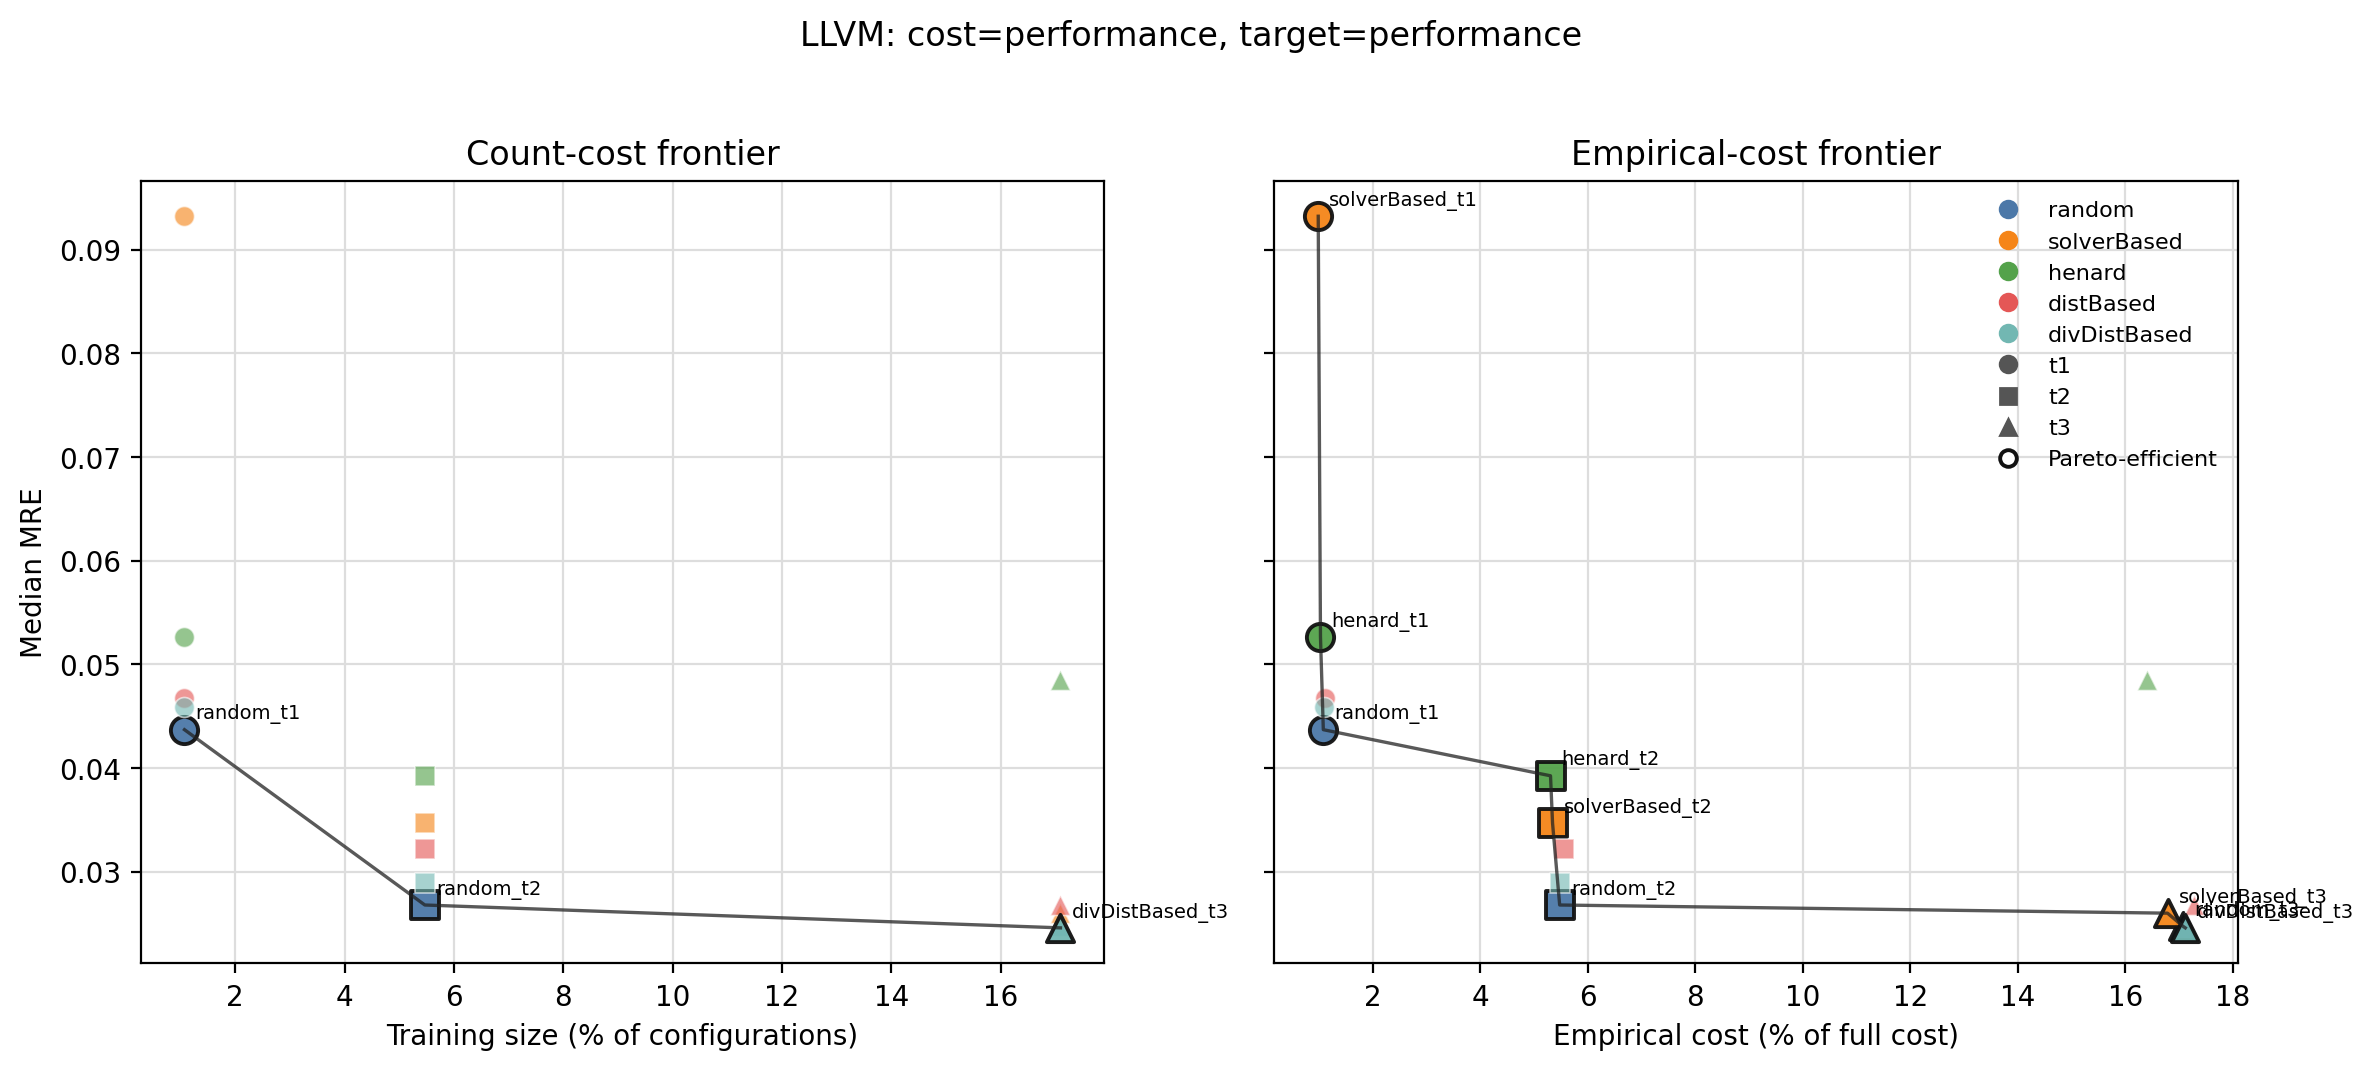
\includegraphics[width=\linewidth]{pic/results/llvm_rq4_frontier.png}
\caption{LLVM: $|F|\!=\!3$ vs $9$.}
\label{fig:rq4-vignette-llvm}
\end{subfigure}\hfill
\begin{subfigure}{0.49\linewidth}
\centering
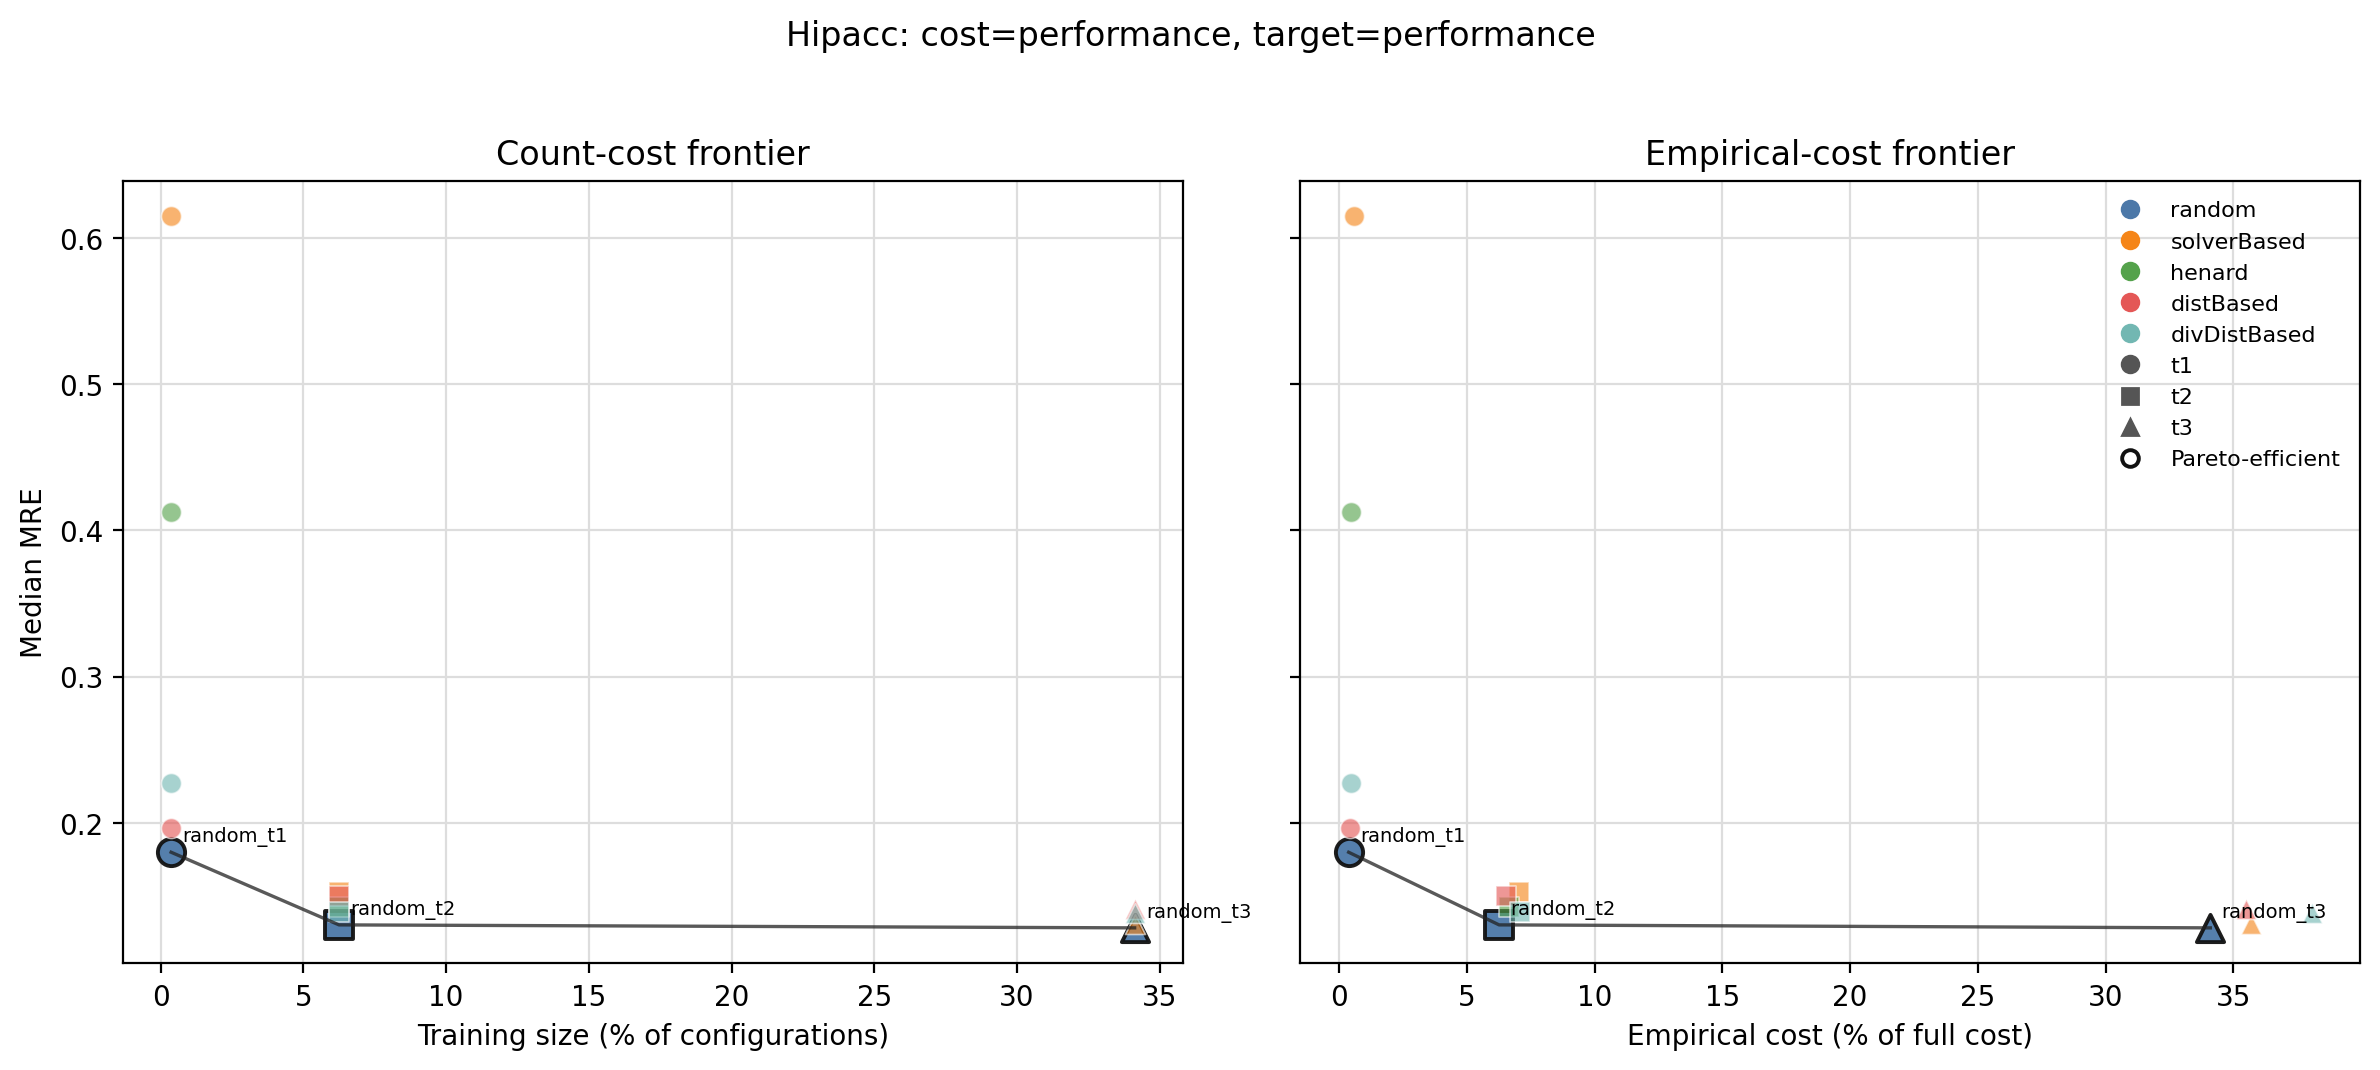
\includegraphics[width=\linewidth]{pic/results/hipacc_rq4_frontier.png}
\caption{HIPAcc: both $|F|\!=\!3$.}
\label{fig:rq4-vignette-hipacc}
\end{subfigure}
\caption{\StudyReplication RQ4 vignette --- count-cost vs empirical-cost
Pareto frontiers.}
\label{fig:rq4-vignettes}
\end{figure}

On x264, median frontier overlap is $0.43$ on time/time and $0.38$
on the asymmetric time/size scenario; per-input range on the worst
scenario is $0.27$--$0.60$ (\Cref{tab:x264-per-input}). Count
frontier contains $3$ pairs on every input; empirical-cost frontier
ranges from $5$ to $11$ pairs.

\begin{figure}[t]
\centering
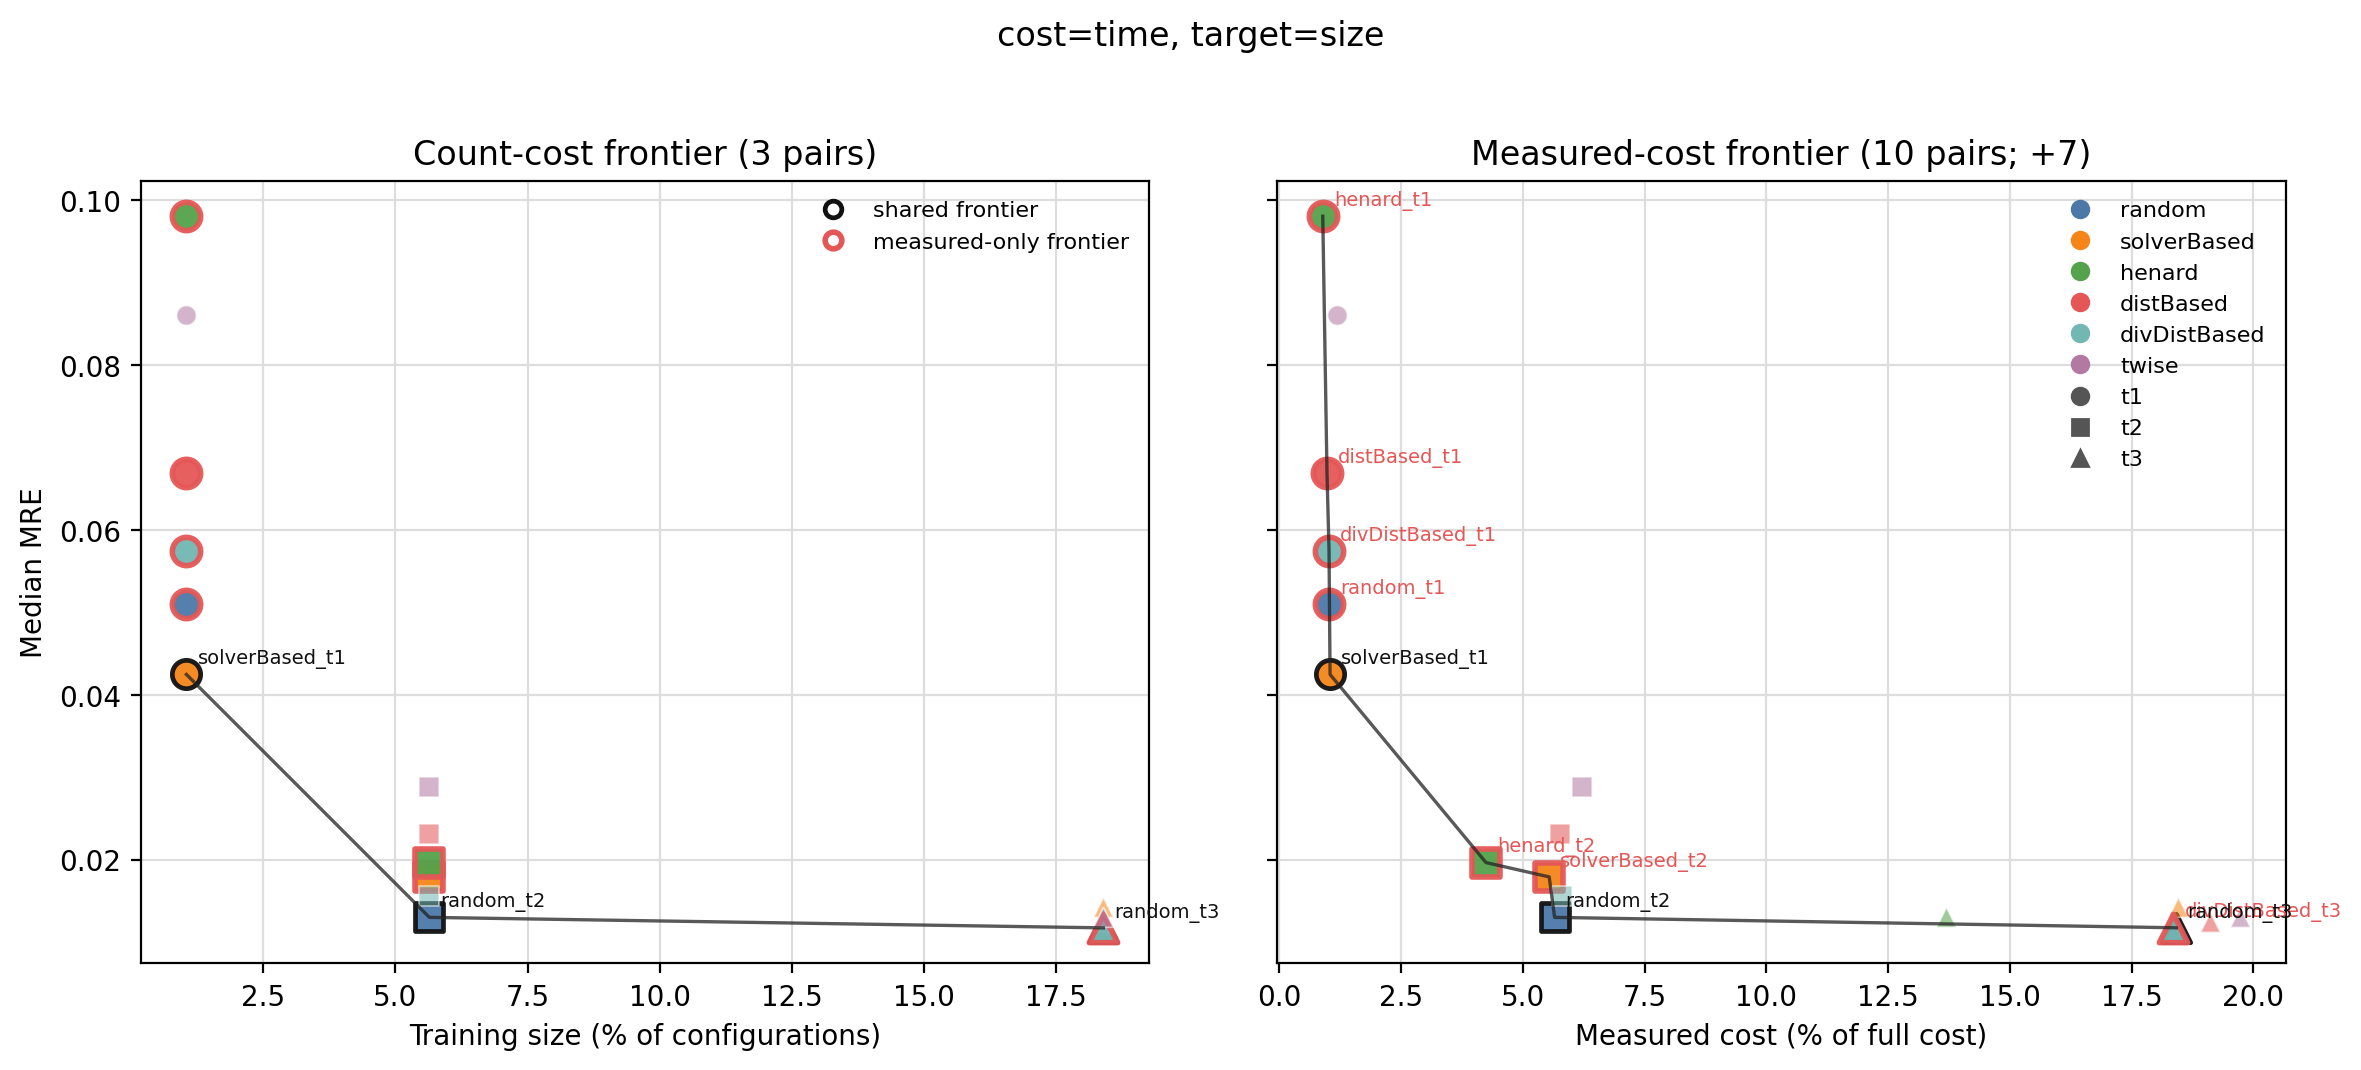
\includegraphics[width=\linewidth]{pic/results/fig_rq4_frontier_cost_time__target_size.png}
\caption{\StudyReplication RQ4 (x264) --- Pareto fronts on the
$(\text{cost}\!=\!\text{time}, \text{target}\!=\!\text{size})$
scenario.}
\label{fig:rq4-x264-frontier}
\end{figure}

\paragraph*{\StudyEnergy.}
On \StudyEnergy, count-cost and empirical-cost Pareto frontiers differ in
\emph{$28/28$} scenarios --- the cleanest decision-level result.
Jaccard ranges from $0.25$ (brotli, lrzip on performance-target
scenarios) to $0.69$ (PostgreSQL, HSQLDB). Empirical frontiers are
generally larger than count frontiers (\eg lrzip: $|F|\!=\!7$ vs
$|F|\!=\!13$ on its performance/performance scenario).
\Cref{fig:twins-rq4-vignettes} contrasts brotli's heavy-tailed
(adverse) frontier with PostgreSQL's nearly homogeneous (benign)
frontier.

\begin{figure}[t]
\centering
\begin{subfigure}{0.49\linewidth}
\centering
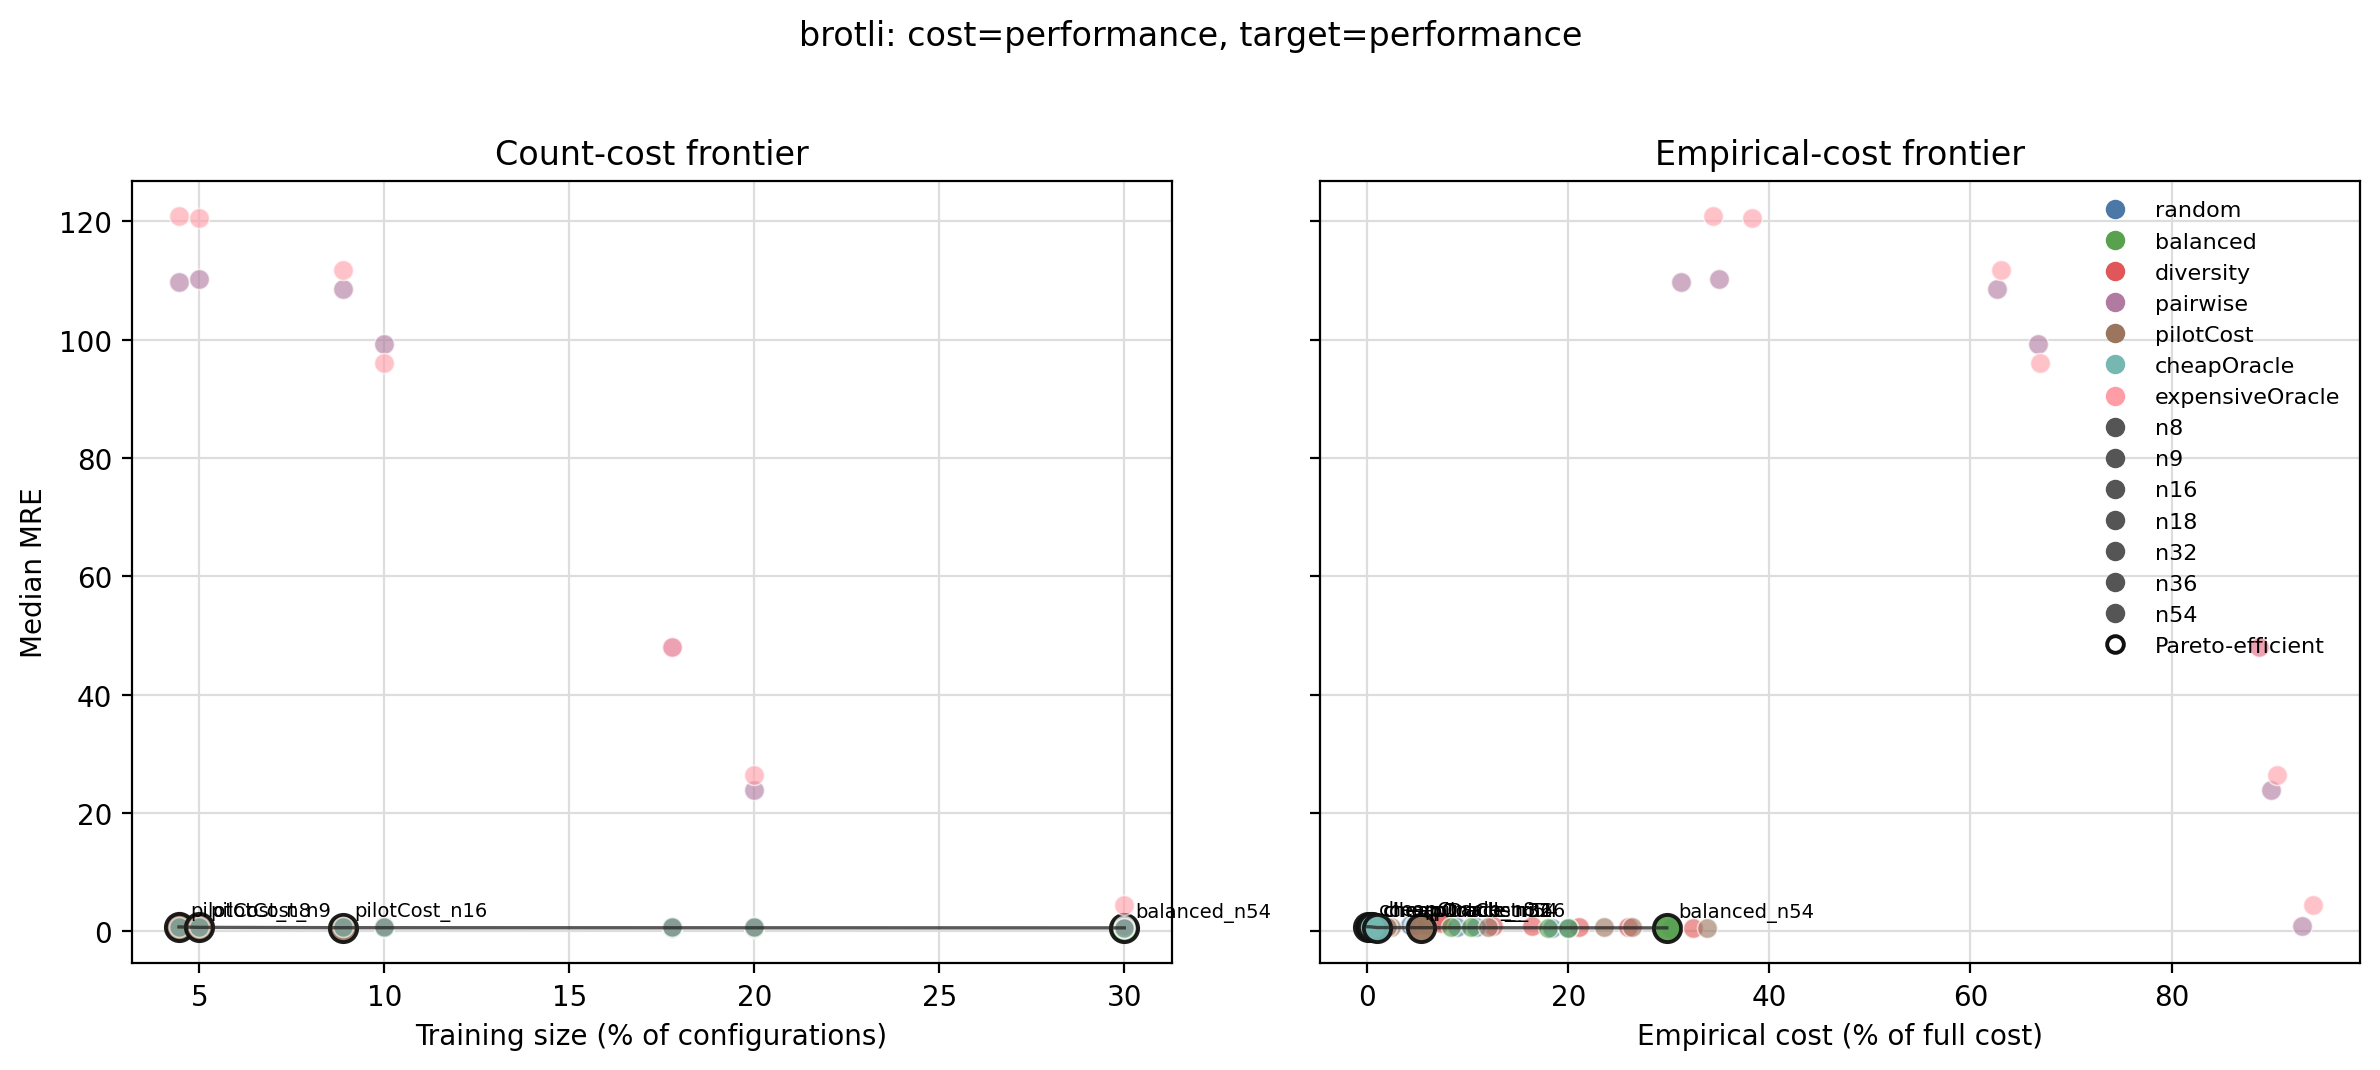
\includegraphics[width=\linewidth]{pic/results/twins_brotli_rq4_frontier.png}
\caption{brotli\,1.0.7 (adverse): Jaccard $0.25$.}
\label{fig:twins-brotli-rq4}
\end{subfigure}\hfill
\begin{subfigure}{0.49\linewidth}
\centering
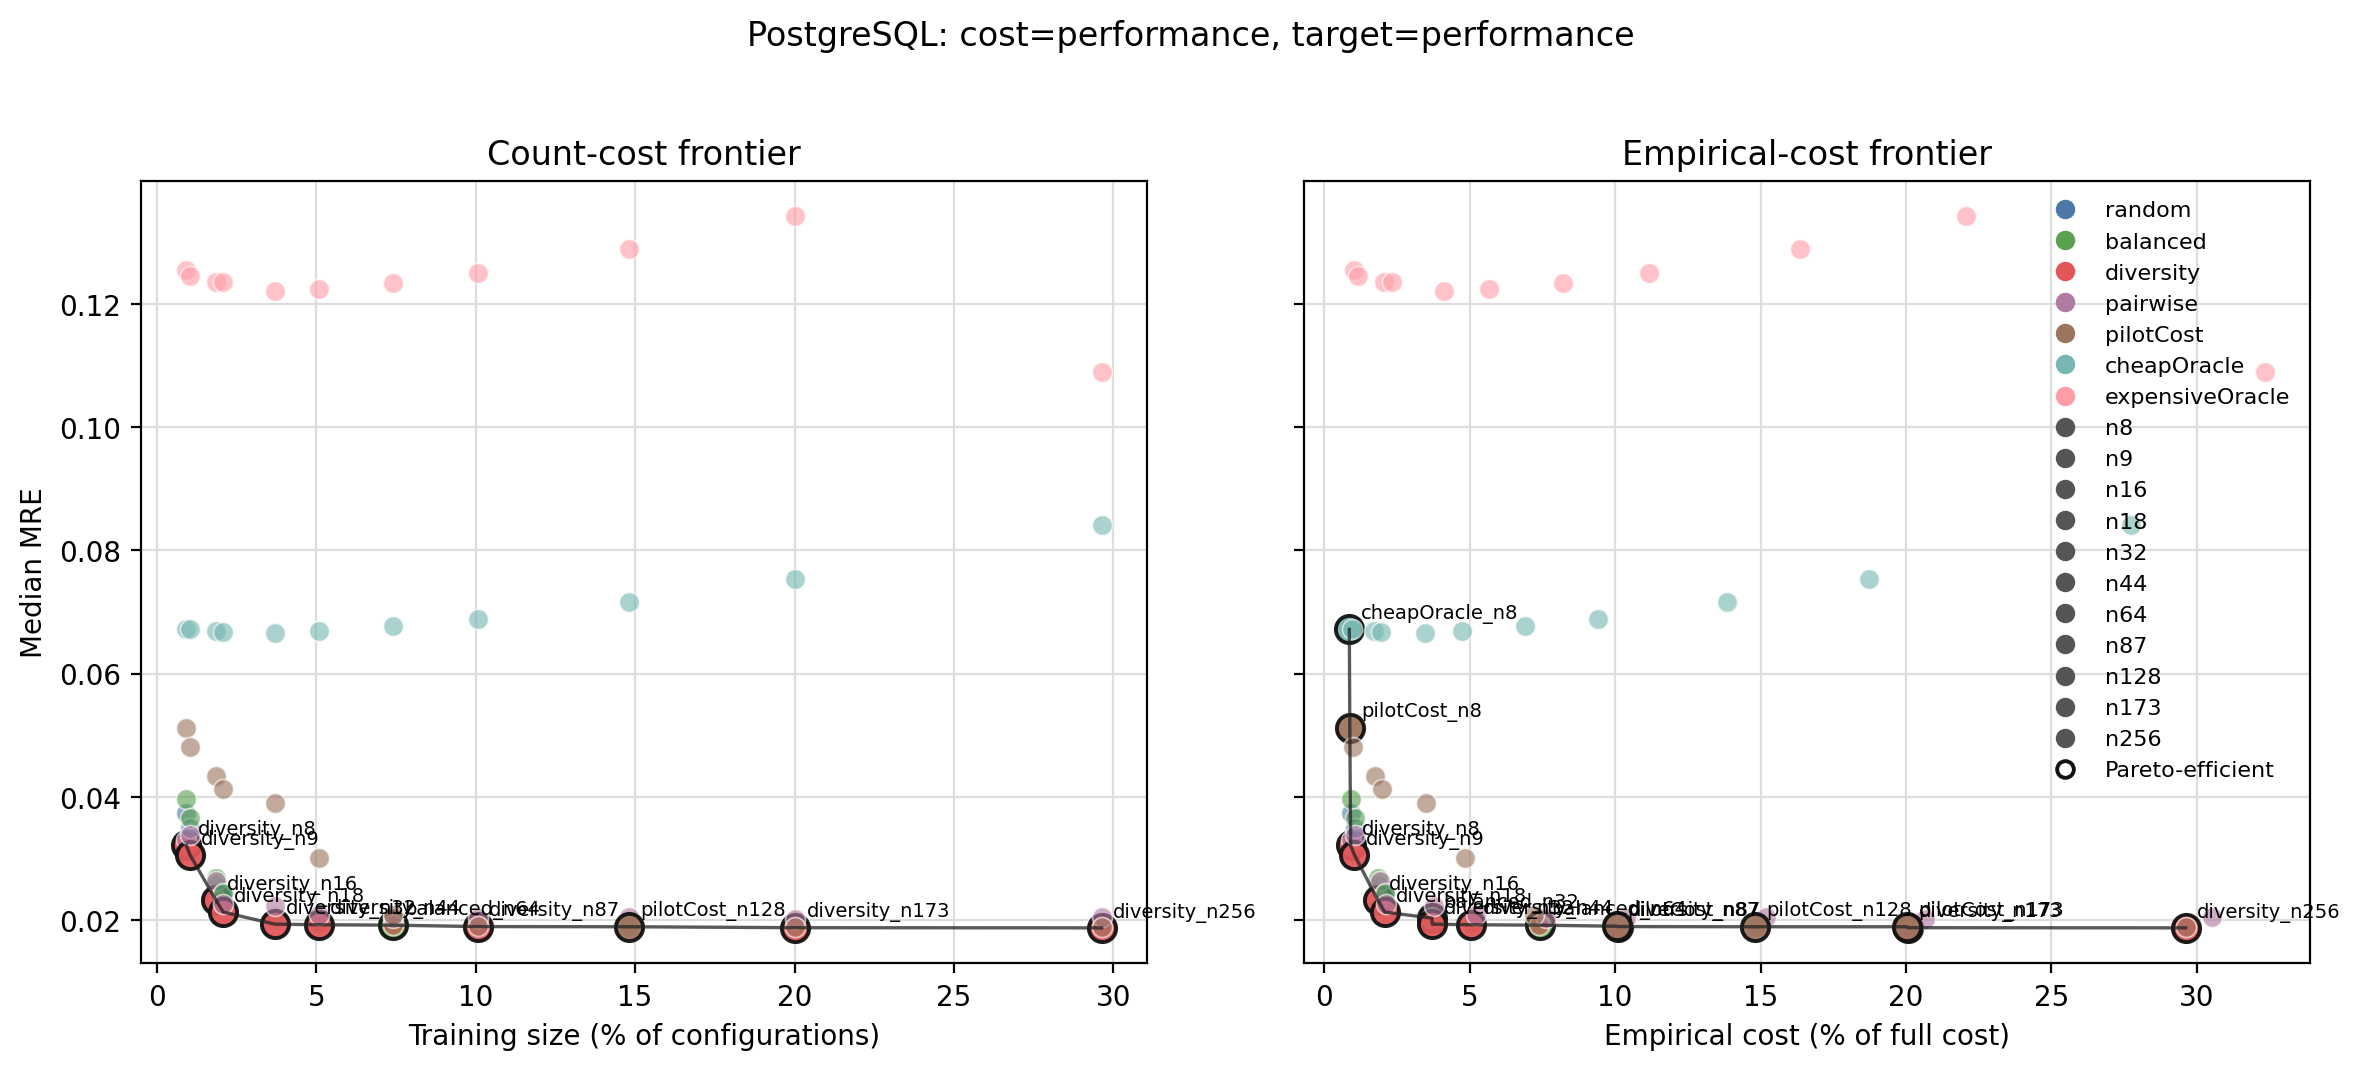
\includegraphics[width=\linewidth]{pic/results/twins_postgres_rq4_frontier.png}
\caption{PostgreSQL\,11.2 (benign): Jaccard $\sim\!\!0.69$.}
\label{fig:twins-postgres-rq4}
\end{subfigure}
\caption{\StudyEnergy RQ4 --- count vs empirical Pareto frontiers on the
performance/performance scenario.}
\label{fig:twins-rq4-vignettes}
\end{figure}

\paragraph*{\StudyWorkload.}
H4b pooled support is $0.81$ across workloads with
$I^{2}\!=\!0.73$. Within-system Pareto Jaccard ranges are wide:
\texttt{xz} $[0.143, 0.500]$, \texttt{x264} $[0.176, 0.500]$,
\texttt{kanzi} $[0.250, 1.000]$, \texttt{dconvert}
$[0.400, 0.750]$. $71/93$ workload contexts have Jaccard $<1$ (the
empirical frontier is strictly larger than the count frontier).
The workload determines whether and by how much the Pareto front
changes, even on systems where the abstract H1a and H2a verdicts
are stable.

\paragraph*{\StudyLinux.}
Empirical Pareto cardinality is $11$ on v4.13 (vs count $5$), $8$ on
v4.15 (vs $6$), $7$ on v5.0 (vs $5$), and $8$ on v5.08 (vs $4$);
Jaccard is $0.45, 0.625, 0.71, 0.50$
(\Cref{fig:linux-rq4-vignettes}). v5.0 has the highest Jaccard
agreement: its small but well-behaved pool produces frontiers that
mostly agree, with only the cheap-tail oracle and one extra
deployable point separating them. \emph{\texttt{diversity} is
Pareto-dominated under both cost models on all seven releases}: it
pays $\sim\!\!2\times$ the cost of \texttt{random} while delivering
$\sim\!\!2\times$ the MRE. Geometric diversity is Pareto-bad on these
pools.

\begin{figure}[t]
\centering
\begin{subfigure}{0.49\linewidth}
\centering
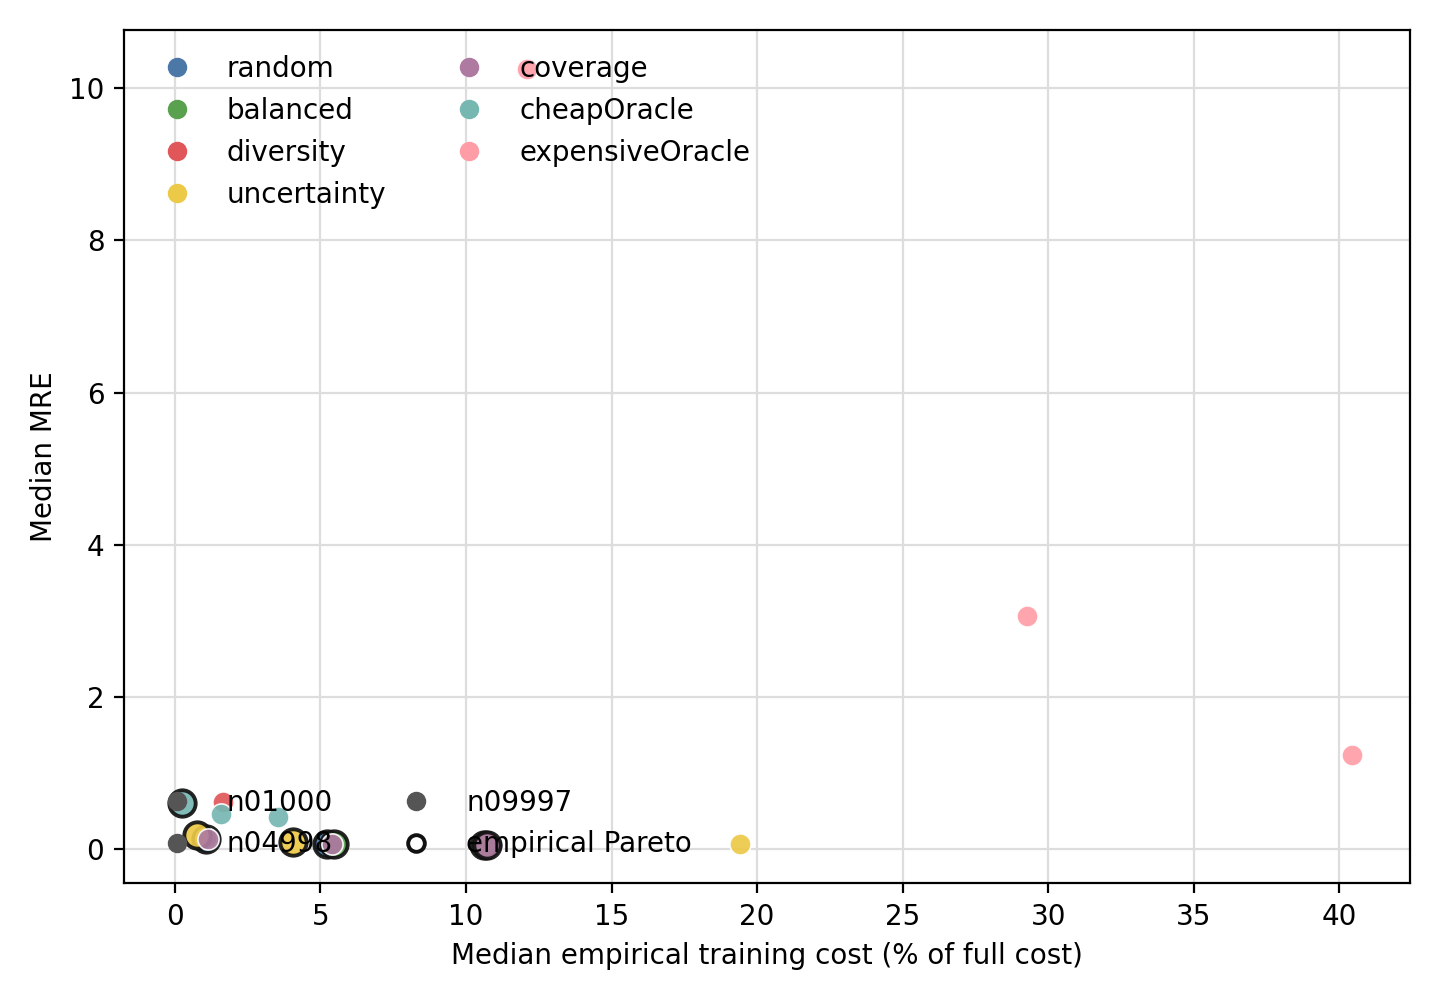
\includegraphics[width=\linewidth]{pic/results/linux413_rq4_frontier.png}
\caption{Linux v4.13: $|F|\!=\!5$ vs $11$.}
\label{fig:linux413-rq4}
\end{subfigure}\hfill
\begin{subfigure}{0.49\linewidth}
\centering
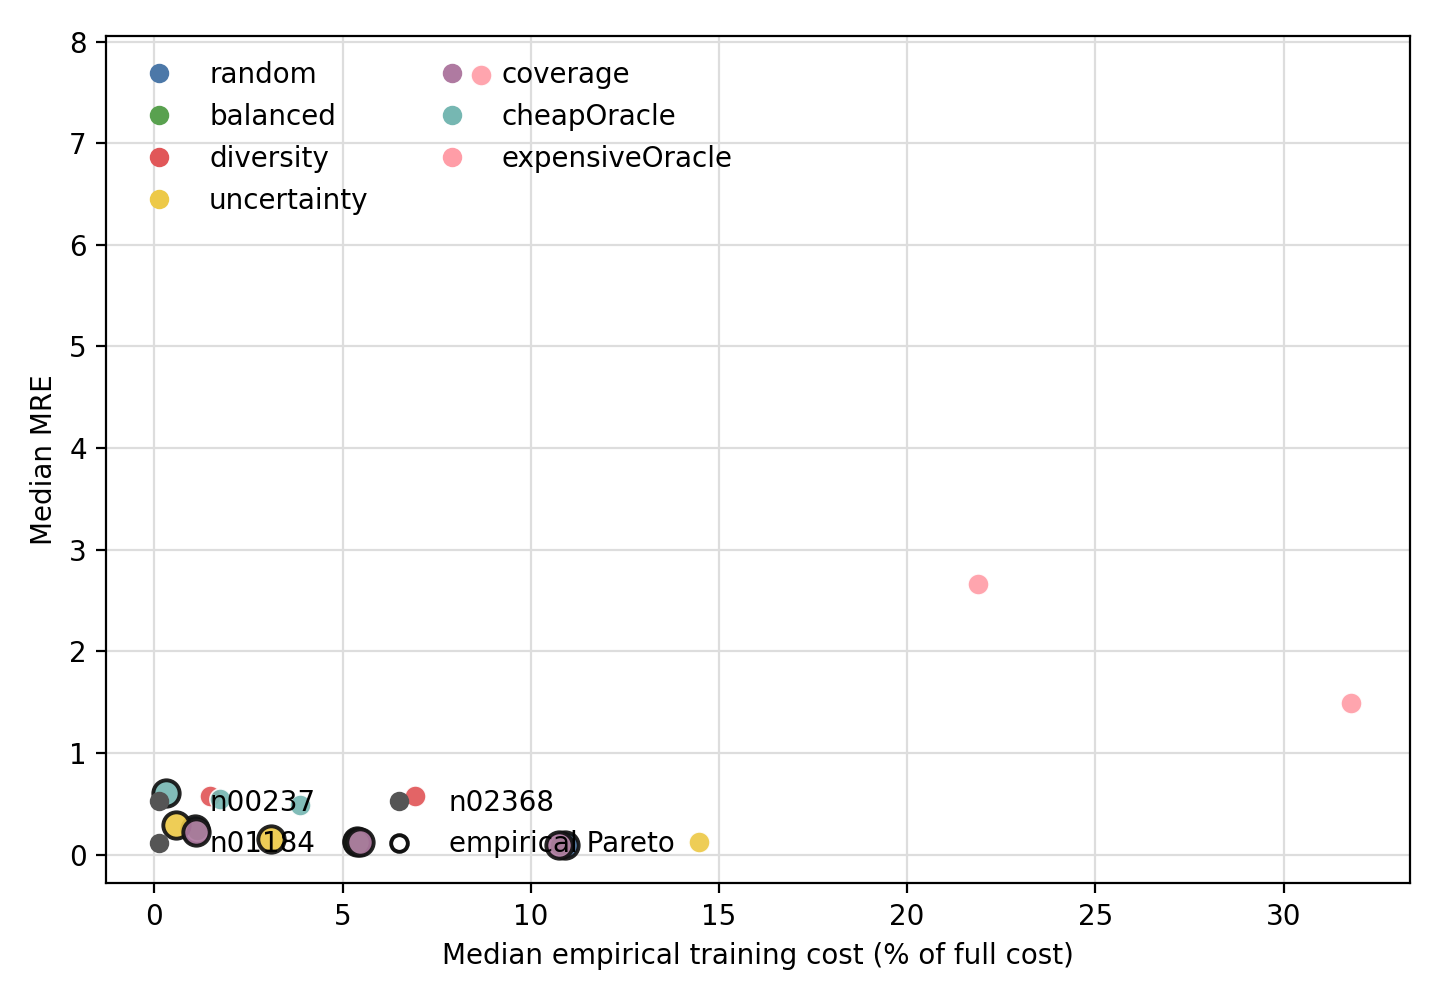
\includegraphics[width=\linewidth]{pic/results/linux508_rq4_frontier.png}
\caption{Linux v5.08: $|F|\!=\!4$ vs $8$.}
\label{fig:linux508-rq4}
\end{subfigure}
\caption{\StudyLinux RQ4 --- count vs empirical Pareto frontiers. On every
release the empirical frontier strictly contains the count frontier.}
\label{fig:linux-rq4-vignettes}
\end{figure}

\rqfinding{RQ4 take-away (cross-family).}{ Pareto Jaccard is
\emph{below $1$ in nearly every scope}: $5/7$ \StudyReplication systems,
$28/28$ \StudyEnergy scenarios, $71/93$ workload contexts, all seven \StudyLinux
releases. The empirical-cost view typically reveals \emph{more}
non-dominated $(s,n)$ pairs than the count view (LLVM $9$ vs $3$;
Linux v4.13 $11$ vs $5$; \StudyEnergy lrzip $13$ vs $7$); size-based
recommendations over-prune the choice space. Crucially, low cost
heterogeneity does not guarantee front stability (LLVM is the
counterexample), and the converse holds too (HIPAcc, Dune,
PostgreSQL).}

\paragraph*{Hypothesis verdicts.}
\textbf{H4a} and \textbf{H4b} are supported in $5/7$ \StudyReplication
systems and $65/68$ x264 input/scenario pairs (\StudyReplication),
$28/28$ \StudyEnergy scenarios (\StudyEnergy), pooled $0.81$ on workloads
($I^{2}\!=\!0.73$, \StudyWorkload), and all seven \StudyLinux releases (\StudyLinux).
The H4 null is rejected as soon as cost is at all heterogeneous,
and the gap is widest exactly where the H3a flips occur, consistent
with H3b within \StudyReplication and \StudyEnergy.

\subsection{RQ5 -- Context Sensitivity}
\label{subsec:results-rq5}

\paragraph*{\StudyReplication.}
The x264 matrix (\Cref{tab:x264-matrix-summary}) exhibits two layers
of context sensitivity. The first is across cost-target scenarios:
under time-cost, swapping the prediction target from time to size
moves top-$1$ agreement from $0.95$ to $0.82$ and median Pareto
Jaccard from $0.43$ to $0.38$. The second is across $17$ x264 inputs
within a single scenario, captured in \Cref{tab:x264-per-input} for
the worst $(\text{cost}\!=\!\text{time}, \text{target}\!=\!\text{size})$
scenario.

\begin{table}[t]
\centering
\caption{\StudyReplication/x264 per-input context sensitivity in the worst
scenario $(\text{cost}\!=\!\text{time}, \text{target}\!=\!\text{size})$.}
\label{tab:x264-per-input}
\footnotesize
\setlength{\tabcolsep}{4pt}
\begin{tabular}{l r r r r r}
\toprule
Input & CV & $p_{90}/p_{10}$ & flips/$7$ & emp.\ Pareto $|F|$ & Jaccard \\
\midrule
$x264_{0}$  & $0.301$ & $2.21$ & $0$ &  $8$ & $0.375$ \\
$x264_{1}$  & $0.258$ & $2.02$ & $0$ &  $6$ & $0.500$ \\
$x264_{2}$  & $0.220$ & $1.81$ & $0$ &  $9$ & $0.333$ \\
$x264_{3}$  & $0.267$ & $2.01$ & $1$ &  $9$ & $0.333$ \\
$x264_{4}$  & $0.230$ & $1.96$ & $2$ & $11$ & $0.273$ \\
$x264_{5}$  & $0.261$ & $2.06$ & $3$ & $10$ & $0.300$ \\
$x264_{6}$  & $0.267$ & $2.05$ & $2$ & $10$ & $0.300$ \\
$x264_{7}$  & $0.247$ & $1.95$ & $0$ &  $9$ & $0.333$ \\
$x264_{8}$  & $0.225$ & $1.86$ & $2$ &  $9$ & $0.333$ \\
$x264_{9}$  & $0.280$ & $2.12$ & $0$ &  $7$ & $0.429$ \\
$x264_{10}$ & $0.249$ & $2.05$ & $0$ &  $6$ & $0.500$ \\
$x264_{11}$ & $0.257$ & $2.07$ & $0$ &  $8$ & $0.375$ \\
$x264_{12}$ & $0.232$ & $1.89$ & $3$ &  $8$ & $0.375$ \\
$x264_{13}$ & $0.212$ & $1.78$ & $0$ &  $7$ & $0.429$ \\
$x264_{14}$ & $0.390$ & $2.98$ & $3$ &  $5$ & $0.600$ \\
$x264_{15}$ & $0.253$ & $1.99$ & $1$ &  $8$ & $0.375$ \\
$x264_{16}$ & $0.248$ & $1.99$ & $4$ & $11$ & $0.273$ \\
\bottomrule
\end{tabular}
\end{table}

\emph{Benign extreme -- $x264_{14}$ (riverbed).} Highest cost CV
($0.390$), $p_{90}/p_{10}\!=\!2.98$, but the \emph{best} Pareto Jaccard
($0.60$): high-motion content produces enough cost spread that the
empirical frontier remains small and largely overlaps the count
frontier.

\emph{Adverse extreme -- $x264_{16}$ (soccer\_4cif).} $4/7$ rank
flips, empirical-cost frontier of $11$ pairs vs count $3$, Jaccard
$0.273$ --- the widest gap, despite a moderate CV ($0.248$).

Across the $17$ inputs, flips/$7$ ranges from $0$ to $4$,
empirical-cost Pareto-front size from $5$ to $11$, Jaccard from
$0.273$ to $0.600$. The aggregate row in
\Cref{tab:x264-matrix-summary} hides per-input variation that is
nearly $2\times$ on Jaccard and $4\times$ on flip count.

\paragraph*{\StudyEnergy.}
On \StudyEnergy, switching the cost property from performance to energy
generally preserves the qualitative direction of the verdict but
shifts magnitudes (CV, calibration ratio, Pareto Jaccard). For
heavy-tailed systems (jump3r, brotli) the shift is stark enough to
change strategy ranks; for near-homogeneous PostgreSQL\,11.2 the
energy and performance verdicts coincide. The cost dimension is a
context variable in its own right.

\paragraph*{\StudyWorkload.}
The $9$-system, $93$-workload corpus is the strongest direct
support for RQ5 (\Cref{tab:workload-impact-meta}). H1a and H2a
travel cleanly across workloads ($86\%, 95\%$ pooled support, low
$I^{2}$), but H2b ($0.33$ pooled, $I^{2}\!=\!0.76$), H3a ($0.80$,
$I^{2}\!=\!0.69$), H4b ($0.81$, $I^{2}\!=\!0.73$) are all
workload-sensitive. A workload-aware variance decomposition
confirms that workload accounts for about $55\%$ of the residual
variance in median calibration ratio and top-$1$ agreement, versus
only $22\%$ for mean Kendall $\tau$.
The system-level extremes are informative: \texttt{xz} supports
H3a and H4b on \emph{all} $13/13$ workloads, while \texttt{lrzip}
supports them on only $2/13$ and $1/13$. \texttt{kanzi} is
intermediate ($3/9$ on H4b). Once a system is fixed, the workload
still materially changes whether the count proxy is miscalibrated
enough to matter and whether a different sampling strategy would be
recommended.

\paragraph*{\StudyLinux.}
The Linux quartet plays the role of cross-version replication:
v4.13, v4.15, v4.20, v5.0, v5.04, v5.07, v5.08 share the same protocol but differ in
pool size and cost-tail heaviness (\Cref{tab:linux-summary}). The
load-bearing observation is that the \emph{calibration regimes
replicate four times} (random/balanced/coverage calibrated;
diversity at $\sim\!\!2\times$; uncertainty $n$-dependent), while
the decision-level verdicts diverge in protocol-driven ways (three
releases at $2/7$ flips, v5.08 at $6/7$ for level-grid reasons).
``Same protocol, different pool'' is therefore a sharper context
sensitivity than ``same pool, different workload'': it isolates
strategy- vs.\ system-level effects that single-pool replication
cannot.

\rqfinding{RQ5 take-away (cross-family).}{ Cost-model validity is
context-dependent in every family, but the \emph{type} of context
that matters depends on the family. On \StudyReplication/x264, the
cost-target scenario alone moves top-$1$ agreement from $0.95$ to
$0.82$ and median Pareto Jaccard from $0.43$ to $0.38$; per-input
within the worst scenario, Jaccard ranges from $0.273$ to $0.600$.
On \StudyEnergy, switching the cost dimension from performance to energy
shifts magnitudes but preserves direction. On \StudyWorkload, workload
accounts for $\sim\!\!55\%$ of within-system variance in
calibration and top-$1$ agreement; some systems are H3a/H4b on
every workload, others on almost none. On \StudyLinux, the calibration
regimes replicate cleanly across seven releases while the
decision-level verdict on v5.08 alone is driven by its level grid,
not by heterogeneity --- a context-sensitivity story that
single-pool replication would have missed entirely. There is no
context-independent answer to ``is $n$ a good proxy?'' in any of
the families.}

\paragraph*{Hypothesis verdicts.}
\textbf{H5a} (input dependence) is supported on the two cost$=$size
scenarios on x264 (Kruskal--Wallis, $\eta^{2}\!=\!0.26$),
inconclusive on the two cost$=$time scenarios. On the workload
batch, H5a system-level summary is supported on $5/9$ systems,
inconclusive on $2/9$, refuted on $2/9$; the workload-level
meta-analysis is the load-bearing evidence.
\textbf{H5b} (target-property gap) is borderline at the by-target
average ($7.95\%$ flip rate predicting time, $12.15\%$ predicting
size, gap $4.2$pp below the $5$-pp pre-registered threshold), but
concentrated in the asymmetric scenario which reaches $17.6\%$
flip rate.
\textbf{H5c} (less-stable rankings under empirical cost) is
supported on the x264 matrix (mean Kendall $\tau\!=\!0.913$, median
Pareto Jaccard $\!=\!0.43$), on all $9$ \dsWLI systems at
the system summary, on \StudyEnergy ($24/28$ scenarios disagree), and on
all seven \StudyLinux releases. The H5c null is rejected.
